%
%
% (c) 2020 Michael Schmid, Hochschule Rapperswil
%
% !TEX root = ../presentation.tex

\begin{frame}
  \frametitle{Linear Convection}
  Propagation of a Wave with constant speed $c$
  $$ \frac{\partial u}{\partial t} + c \frac{\partial u}{\partial x} = 0 $$
\end{frame}

  % \begin{frame}
  %   \frametitle{Linear Convection}
  %   \begin{center}
  %           \includemedia[width=1\linewidth,height=.5\linewidth,activate=pageopen, passcontext, transparent, addresource=slides/images/Linear_Convection.mp4, flashvars={source=slides/images/Linear_Convection.mp4}]{}{VPlayer.swf}
  %   \end{center}
  % \end{frame}

  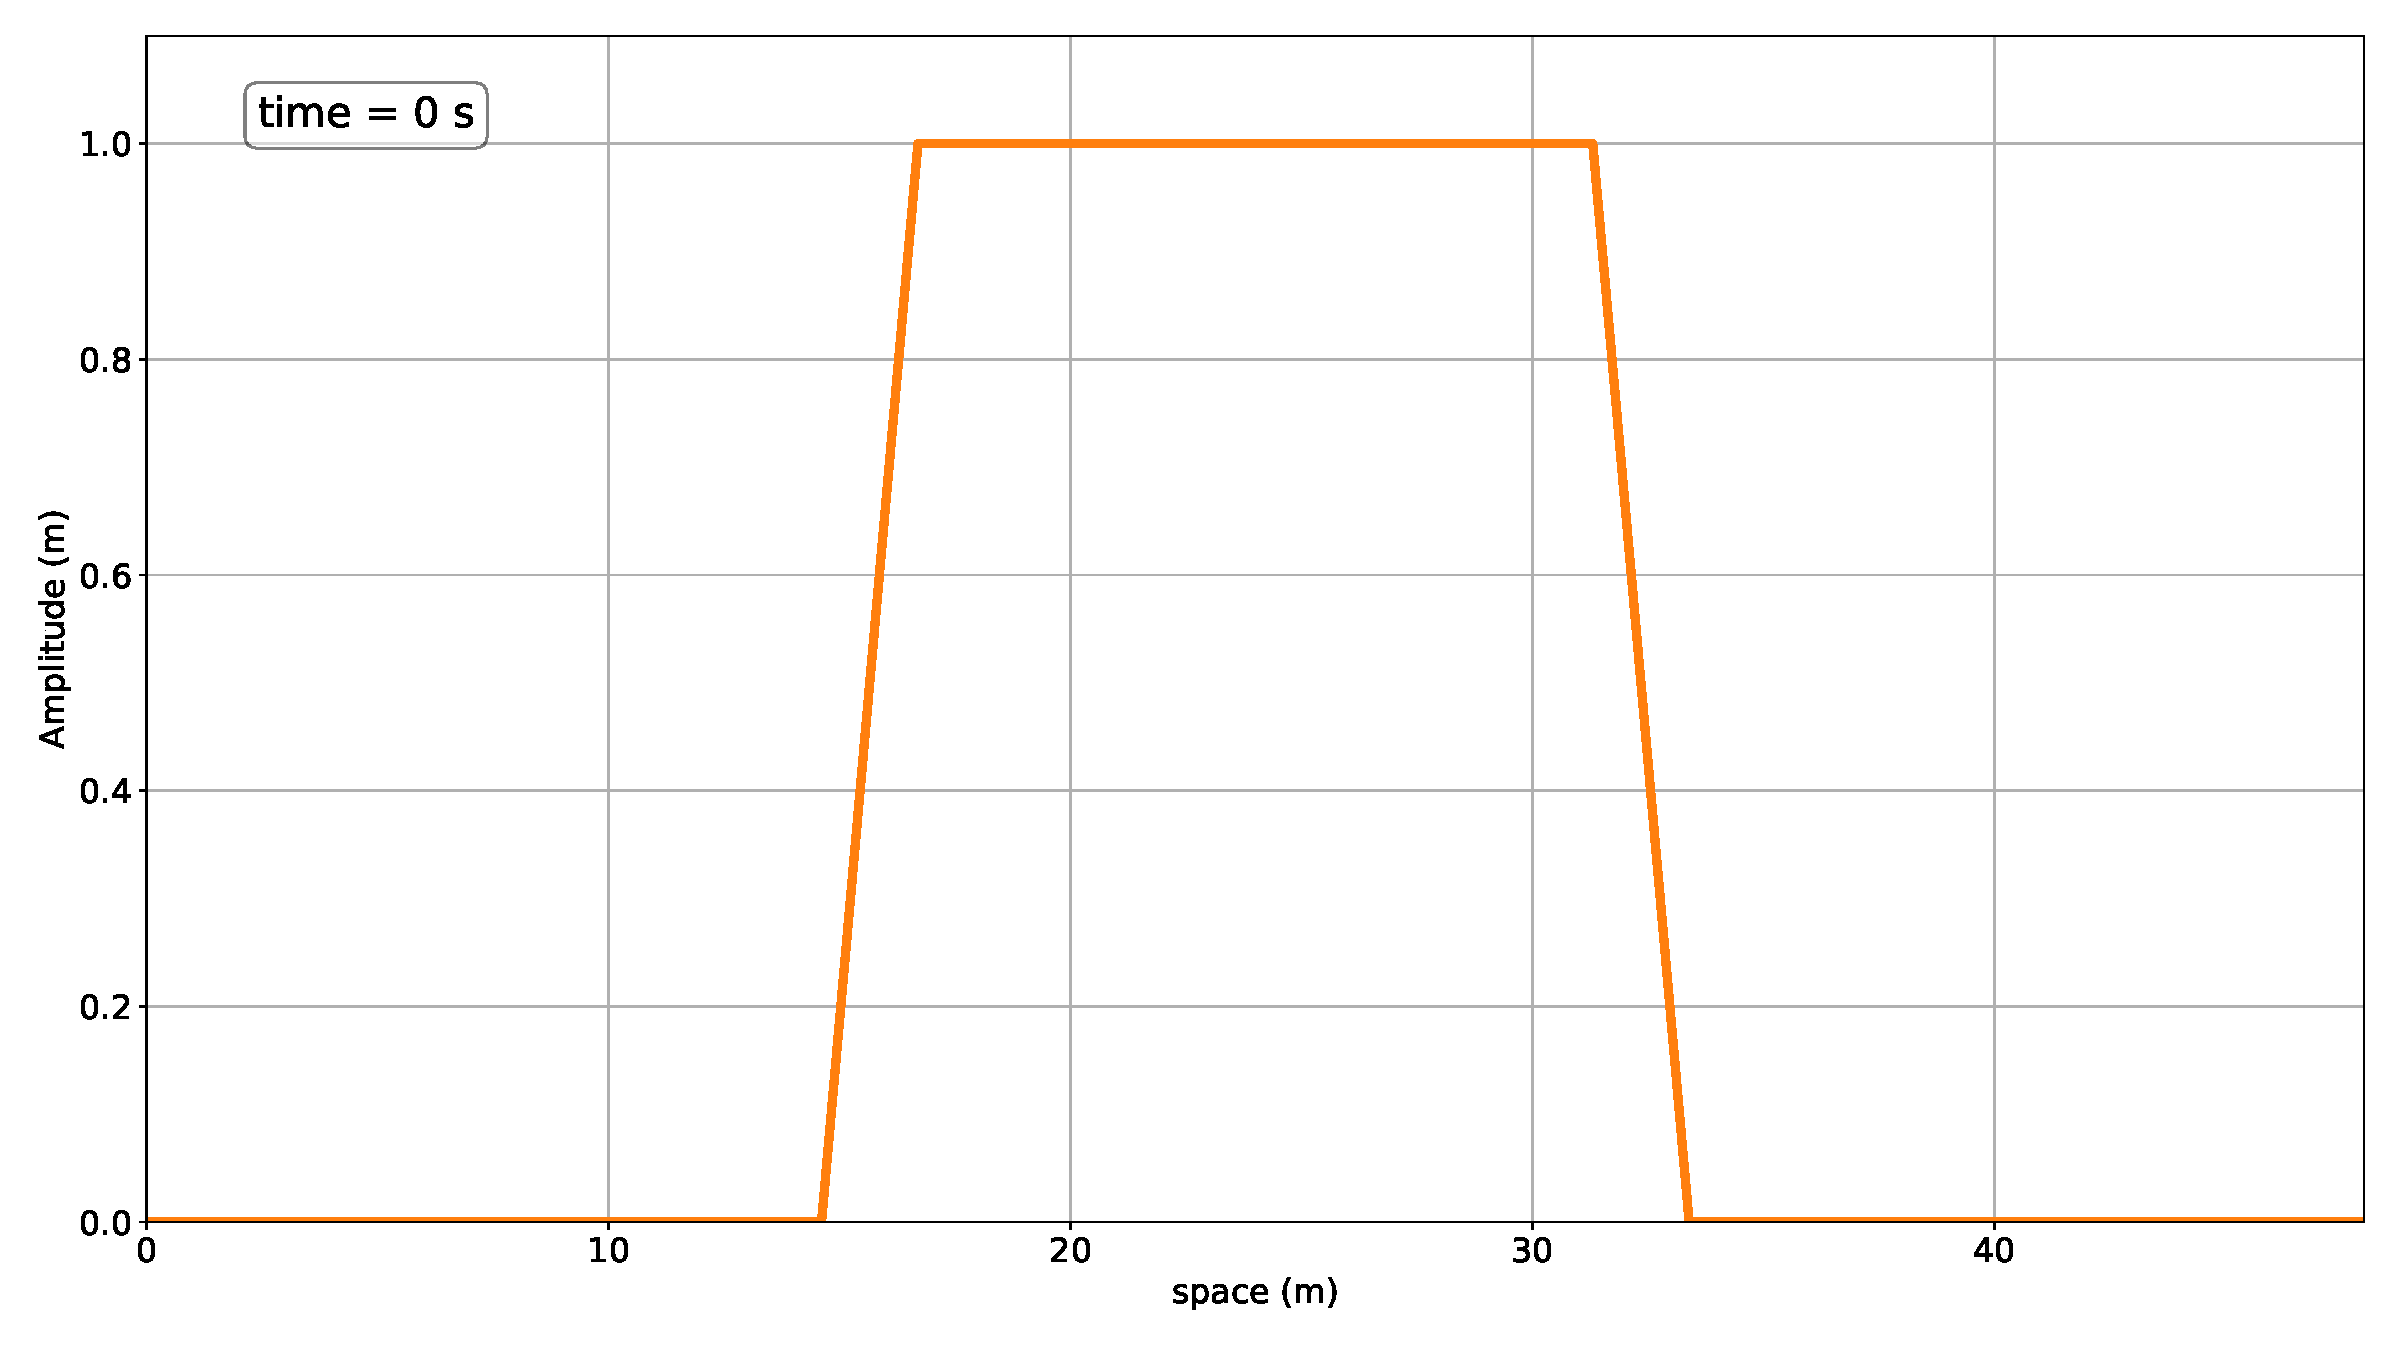
\includegraphics[width=\linewidth]{../BurgersEquation/images/Linear_Convection0.pdf}
  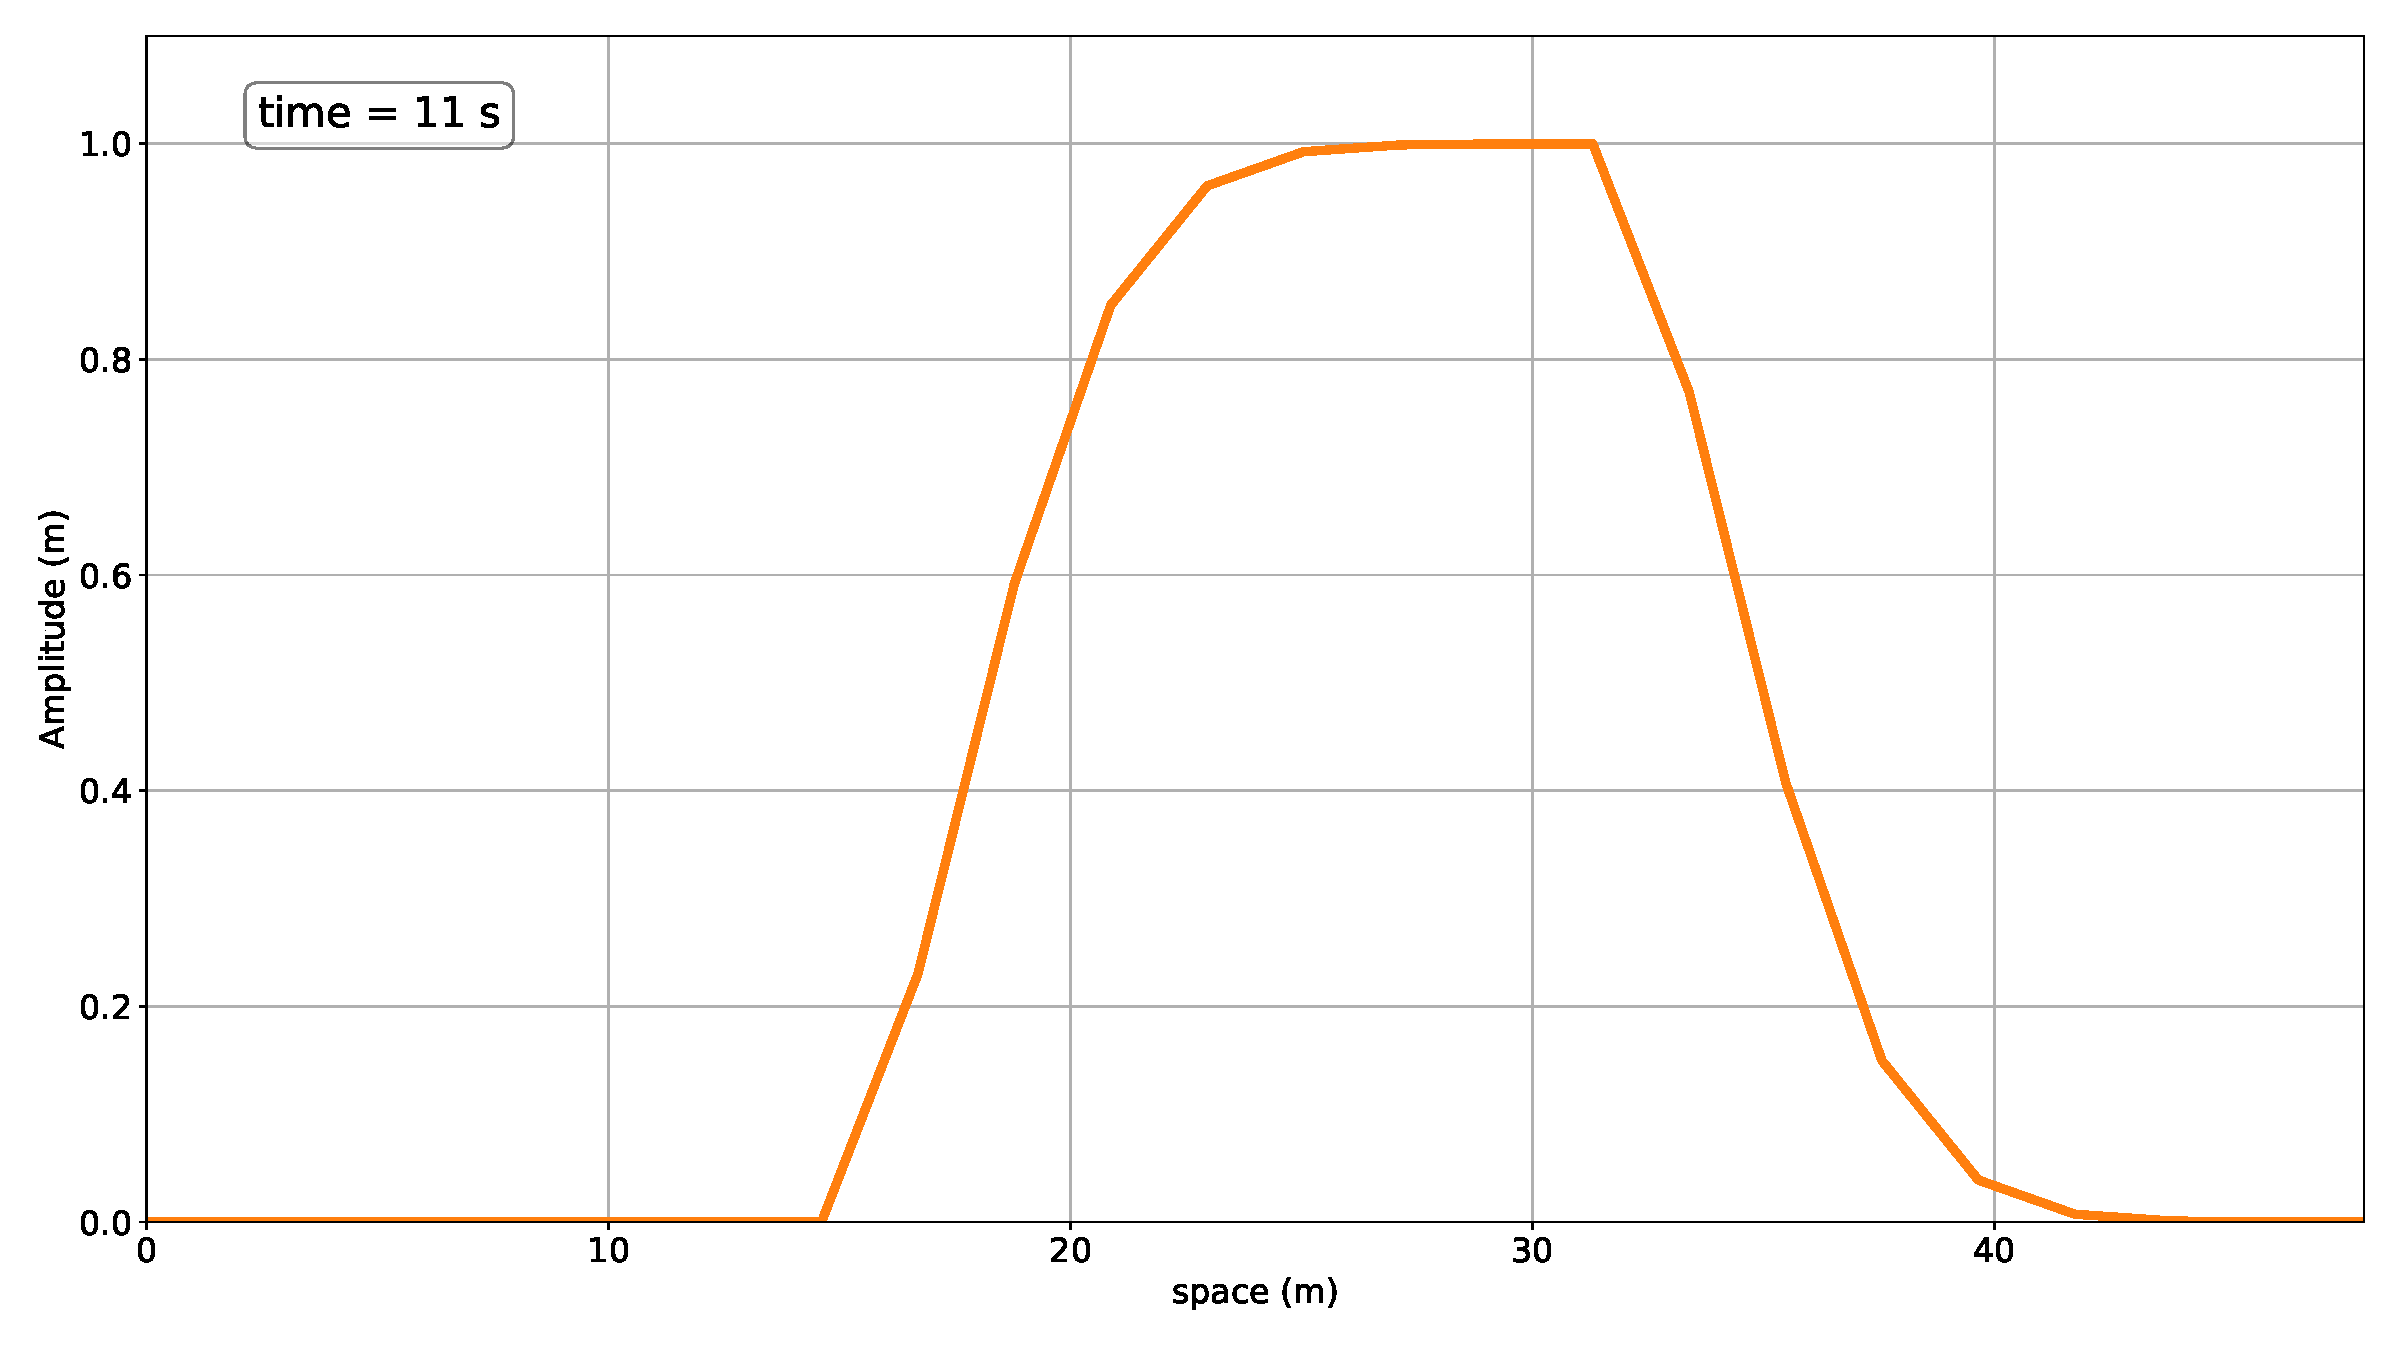
\includegraphics[width=\linewidth]{../BurgersEquation/images/Linear_Convection1.pdf}
  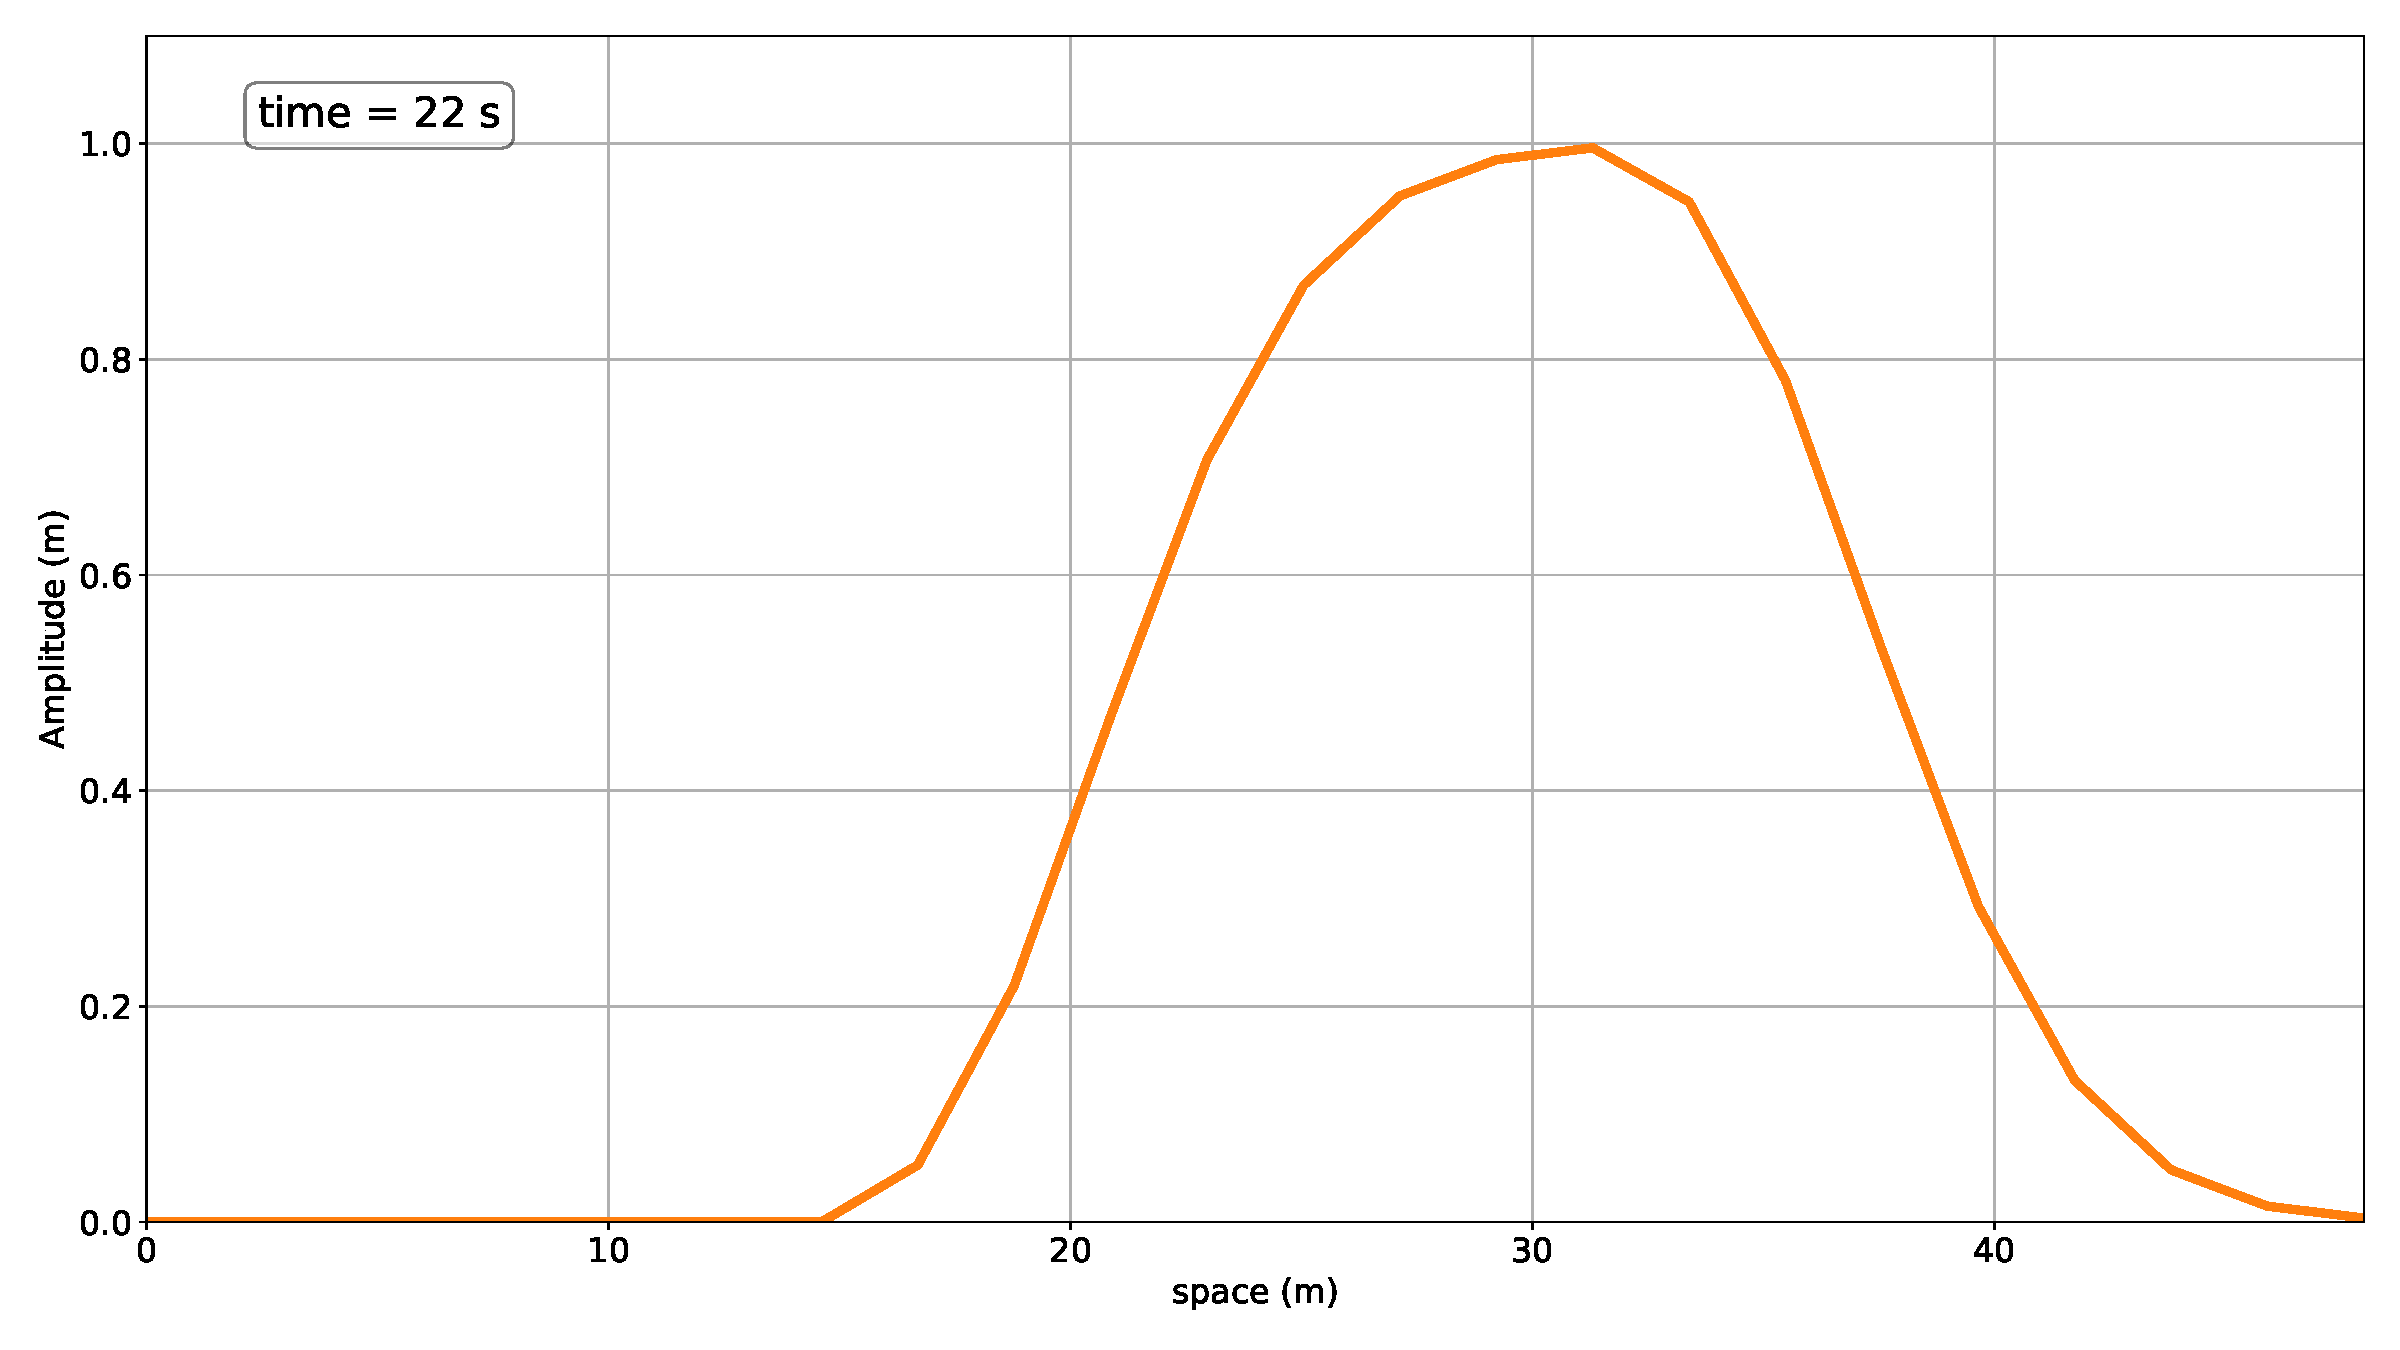
\includegraphics[width=\linewidth]{../BurgersEquation/images/Linear_Convection2.pdf}
  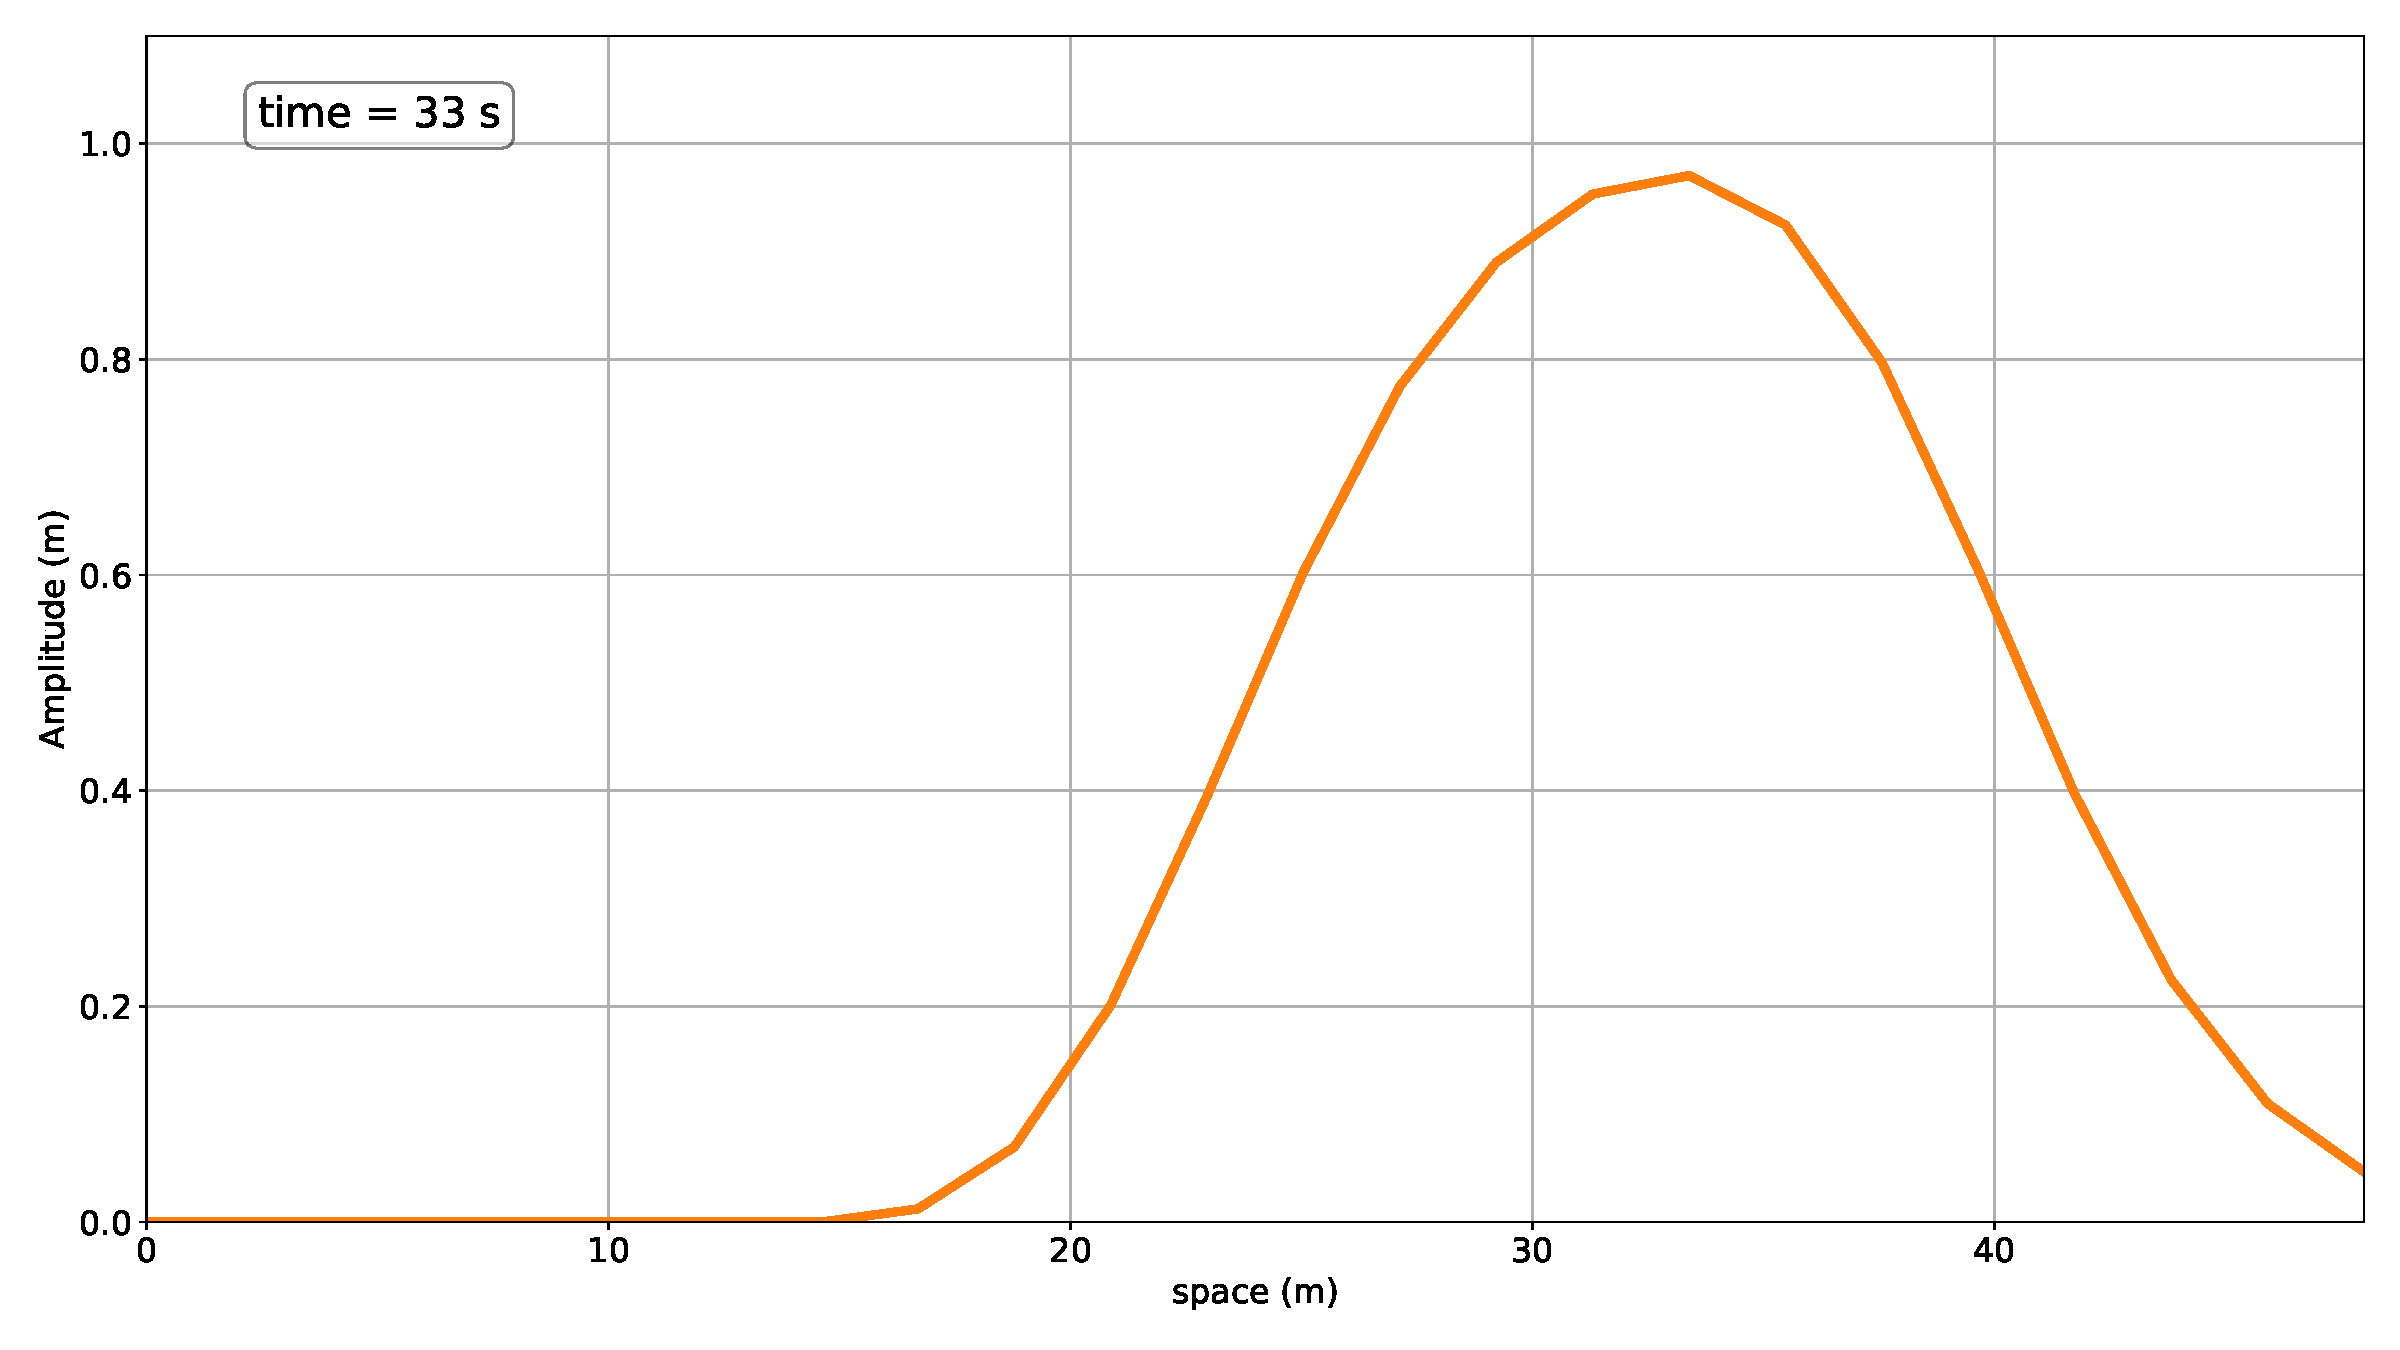
\includegraphics[width=\linewidth]{../BurgersEquation/images/Linear_Convection3.pdf}
  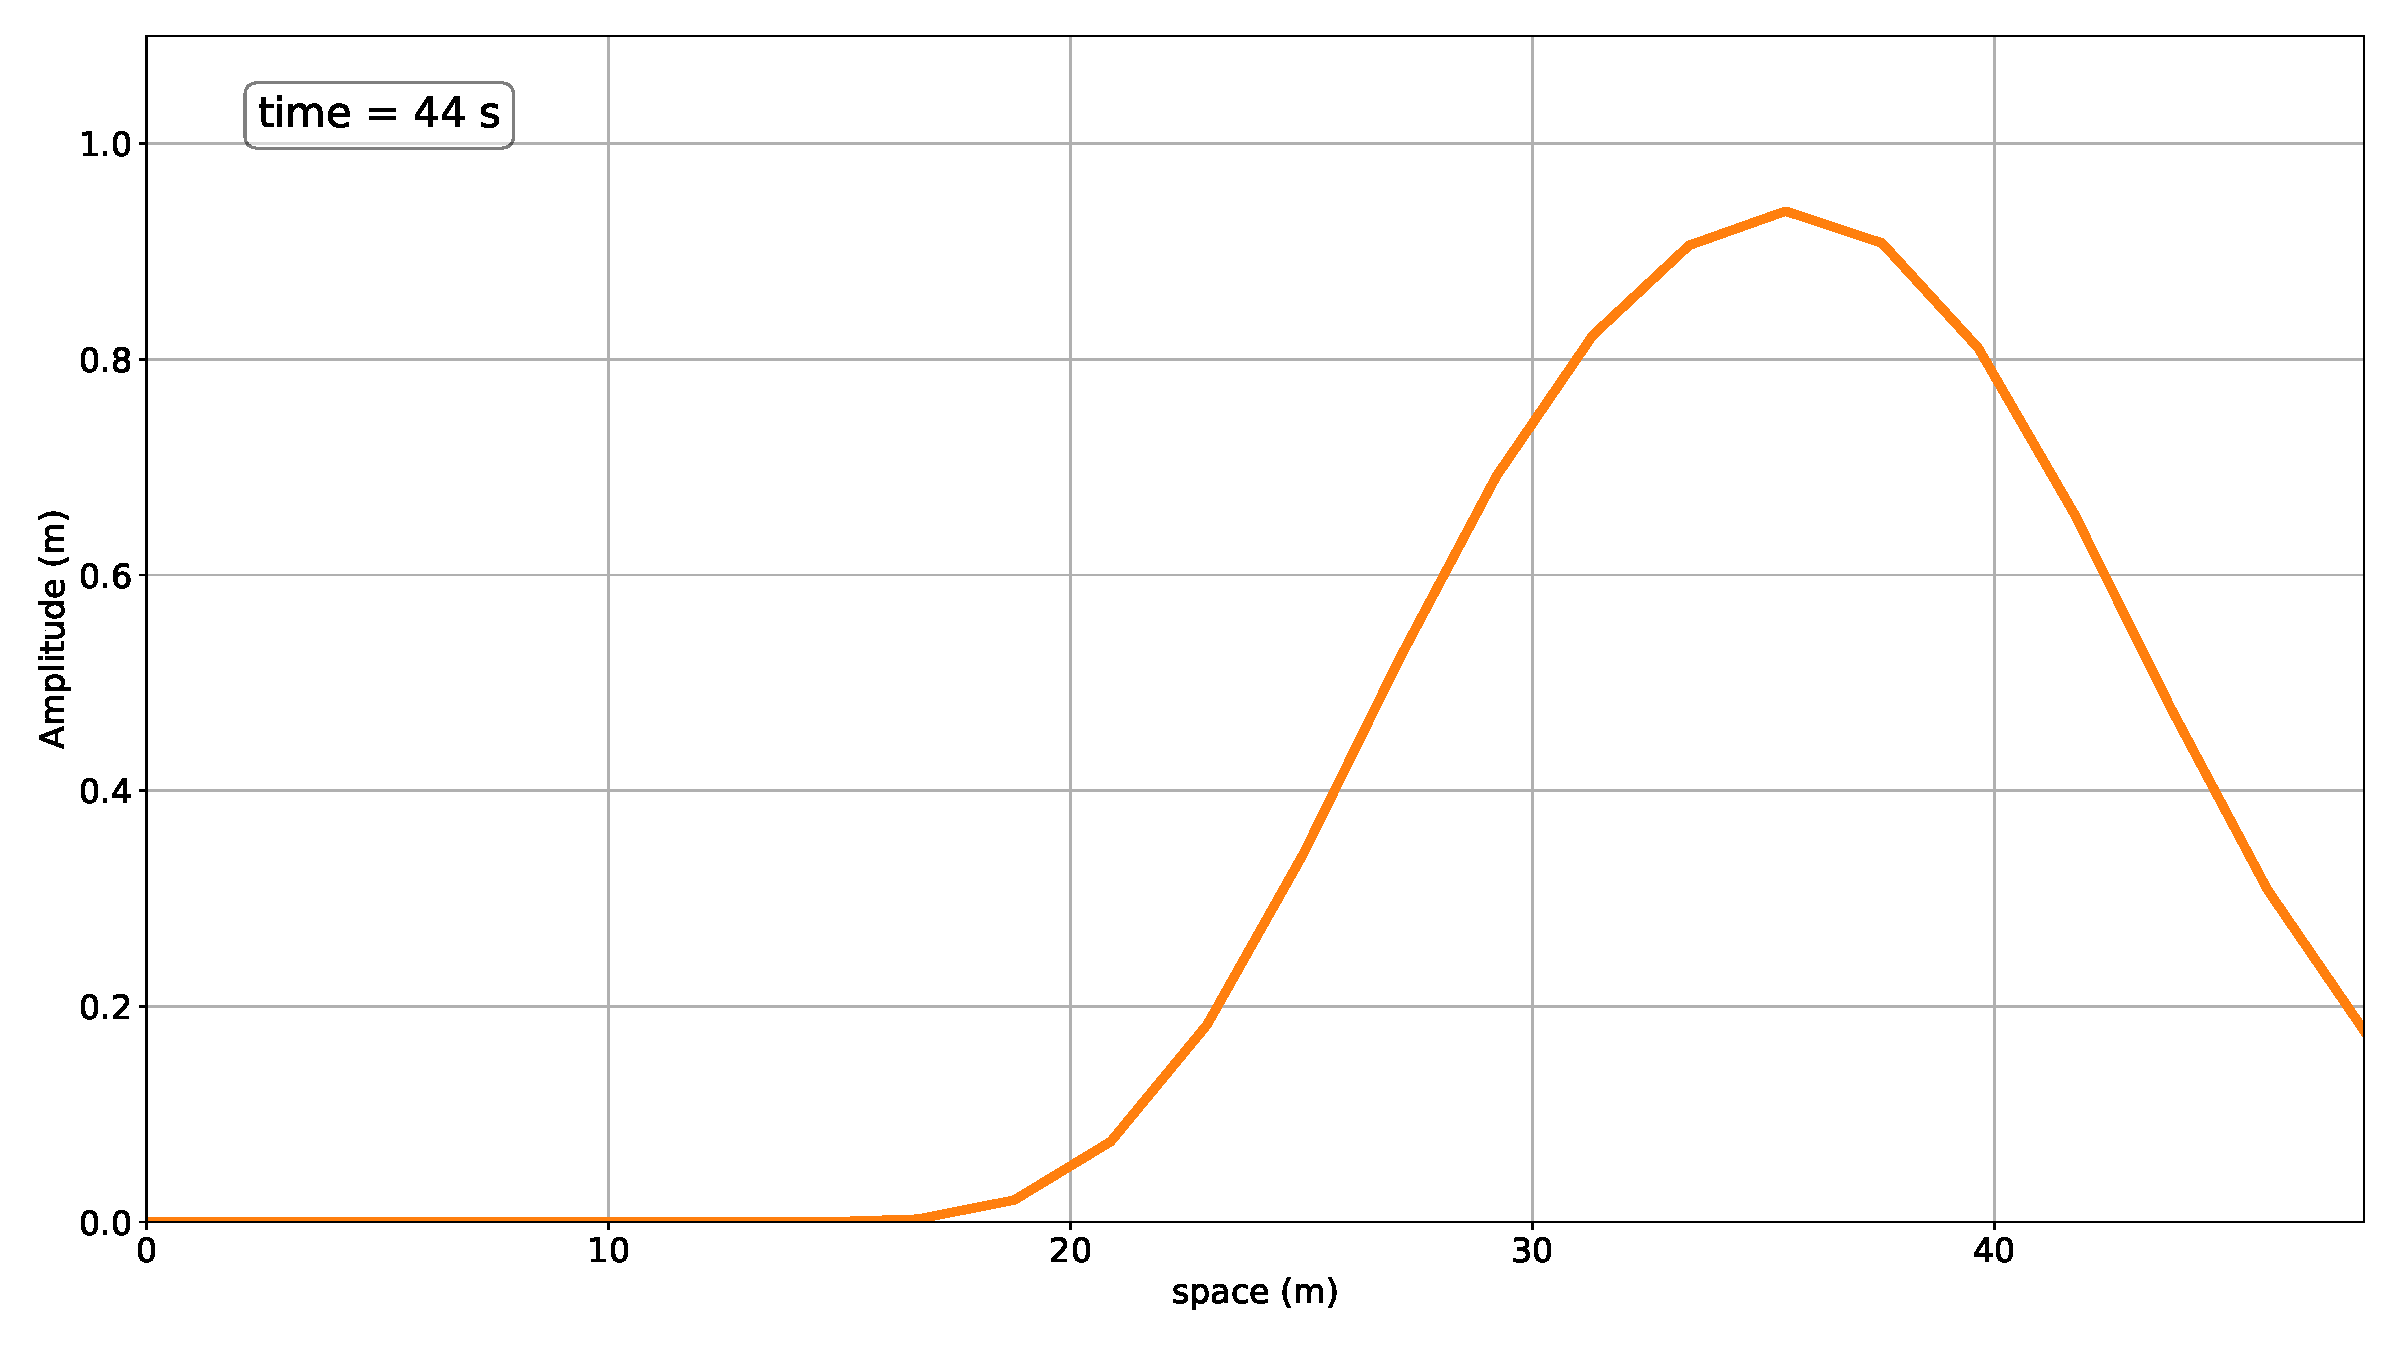
\includegraphics[width=\linewidth]{../BurgersEquation/images/Linear_Convection4.pdf}
  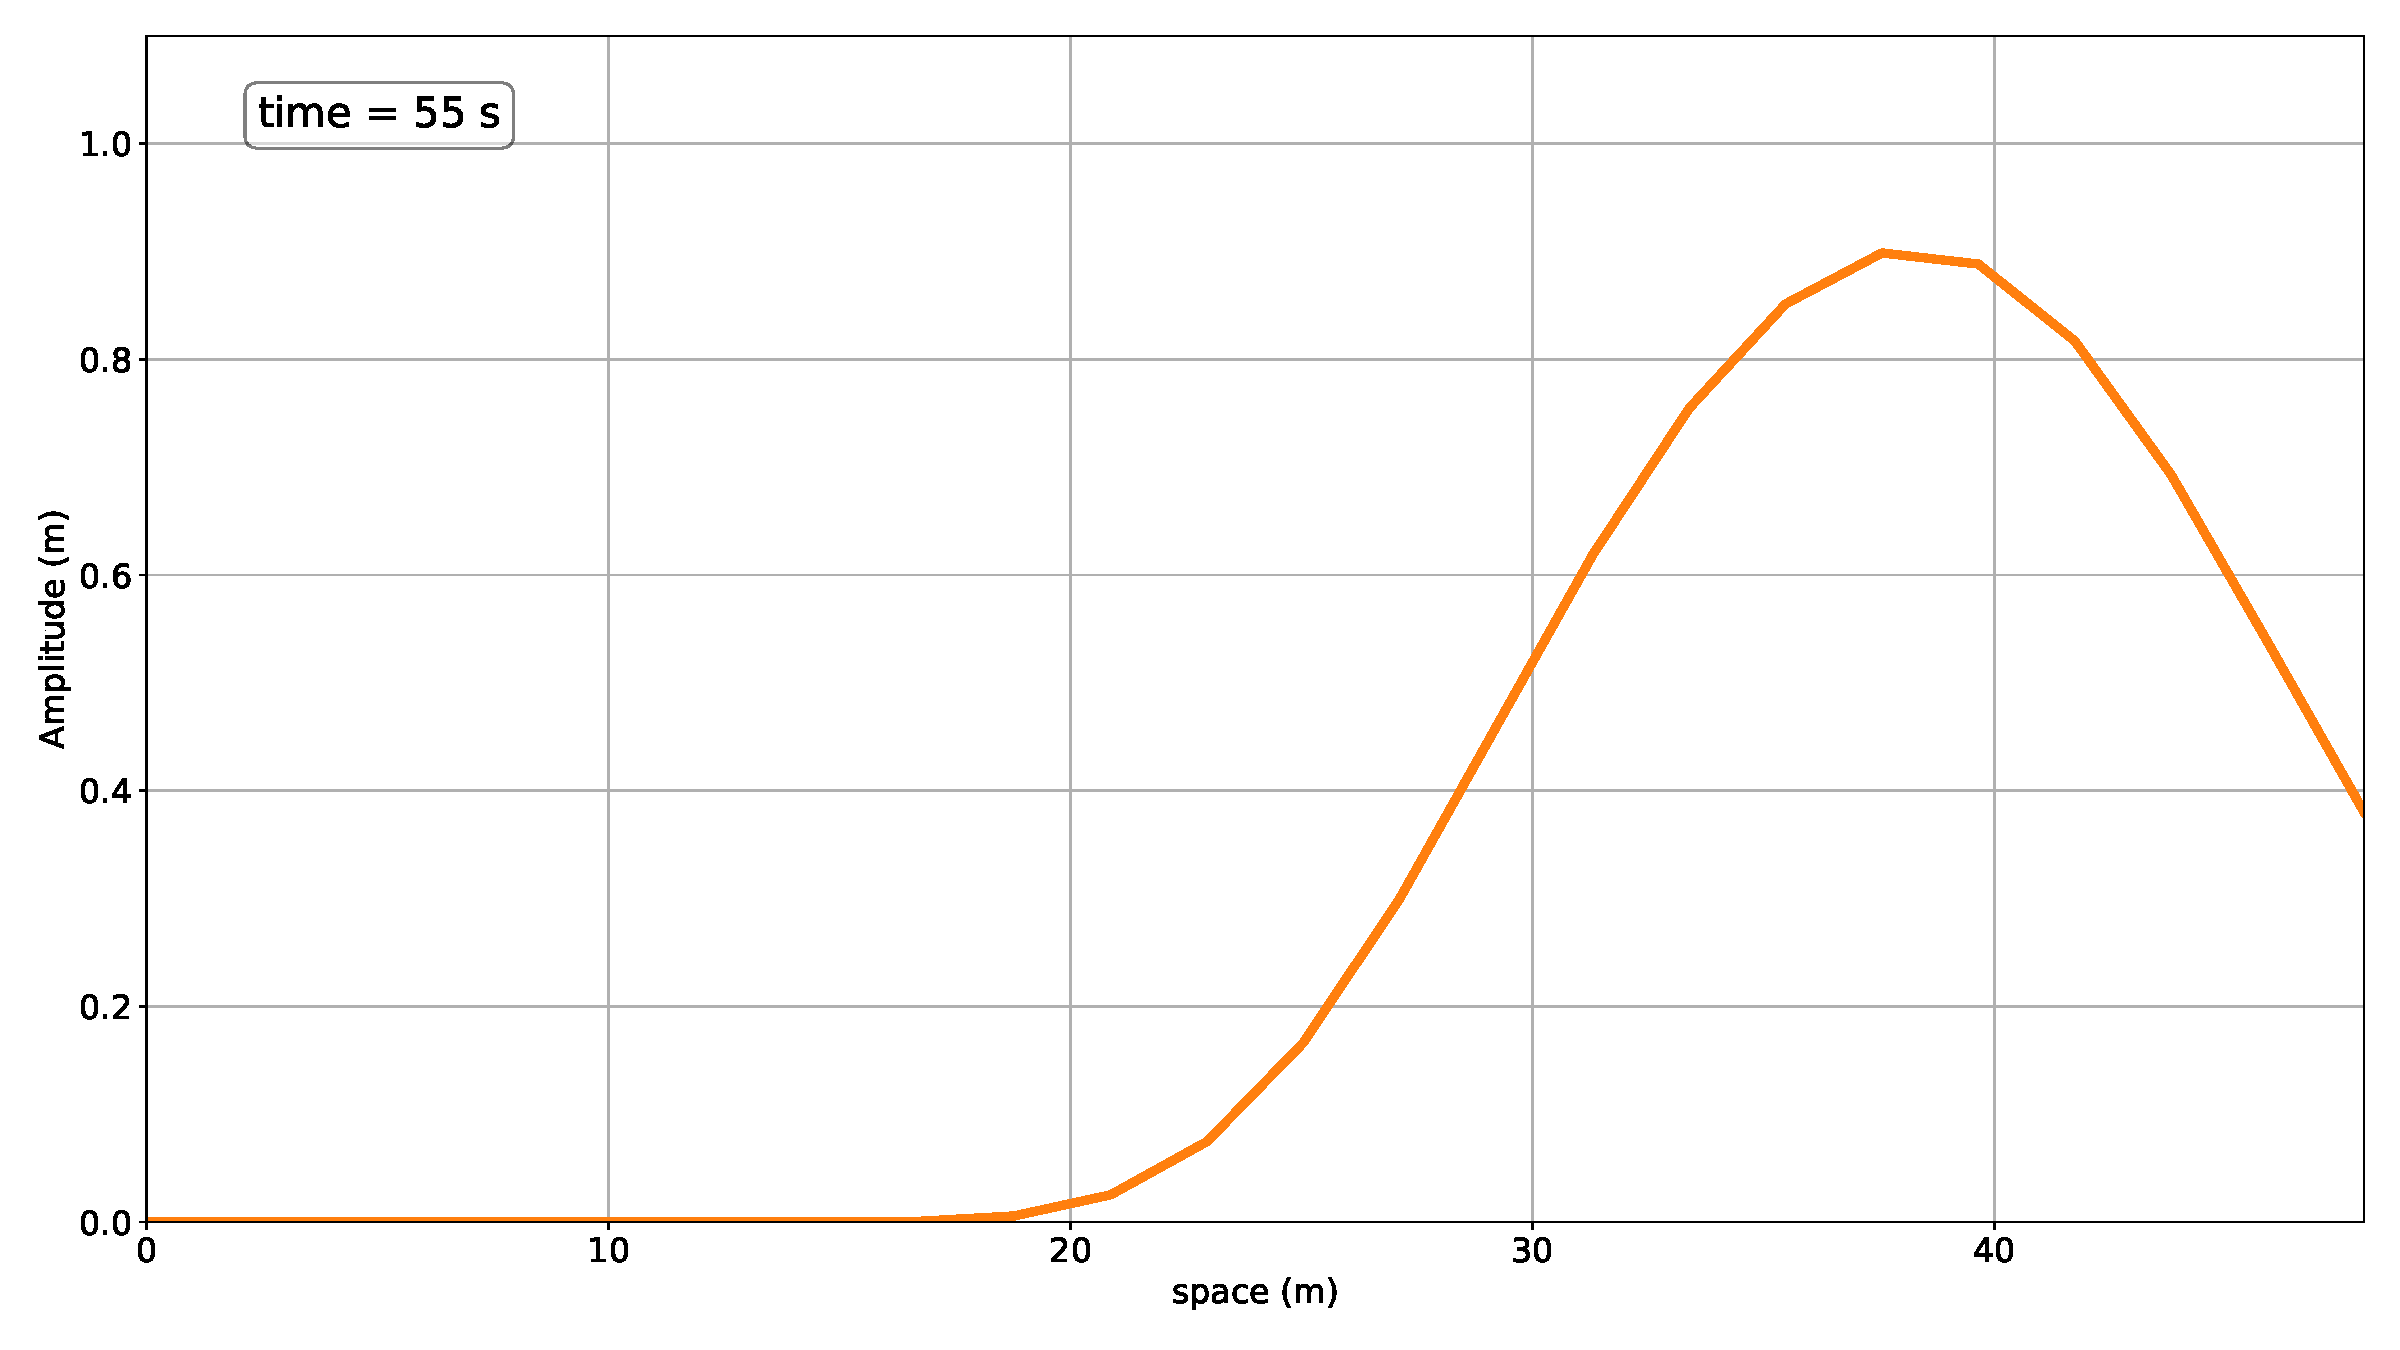
\includegraphics[width=\linewidth]{../BurgersEquation/images/Linear_Convection5.pdf}
  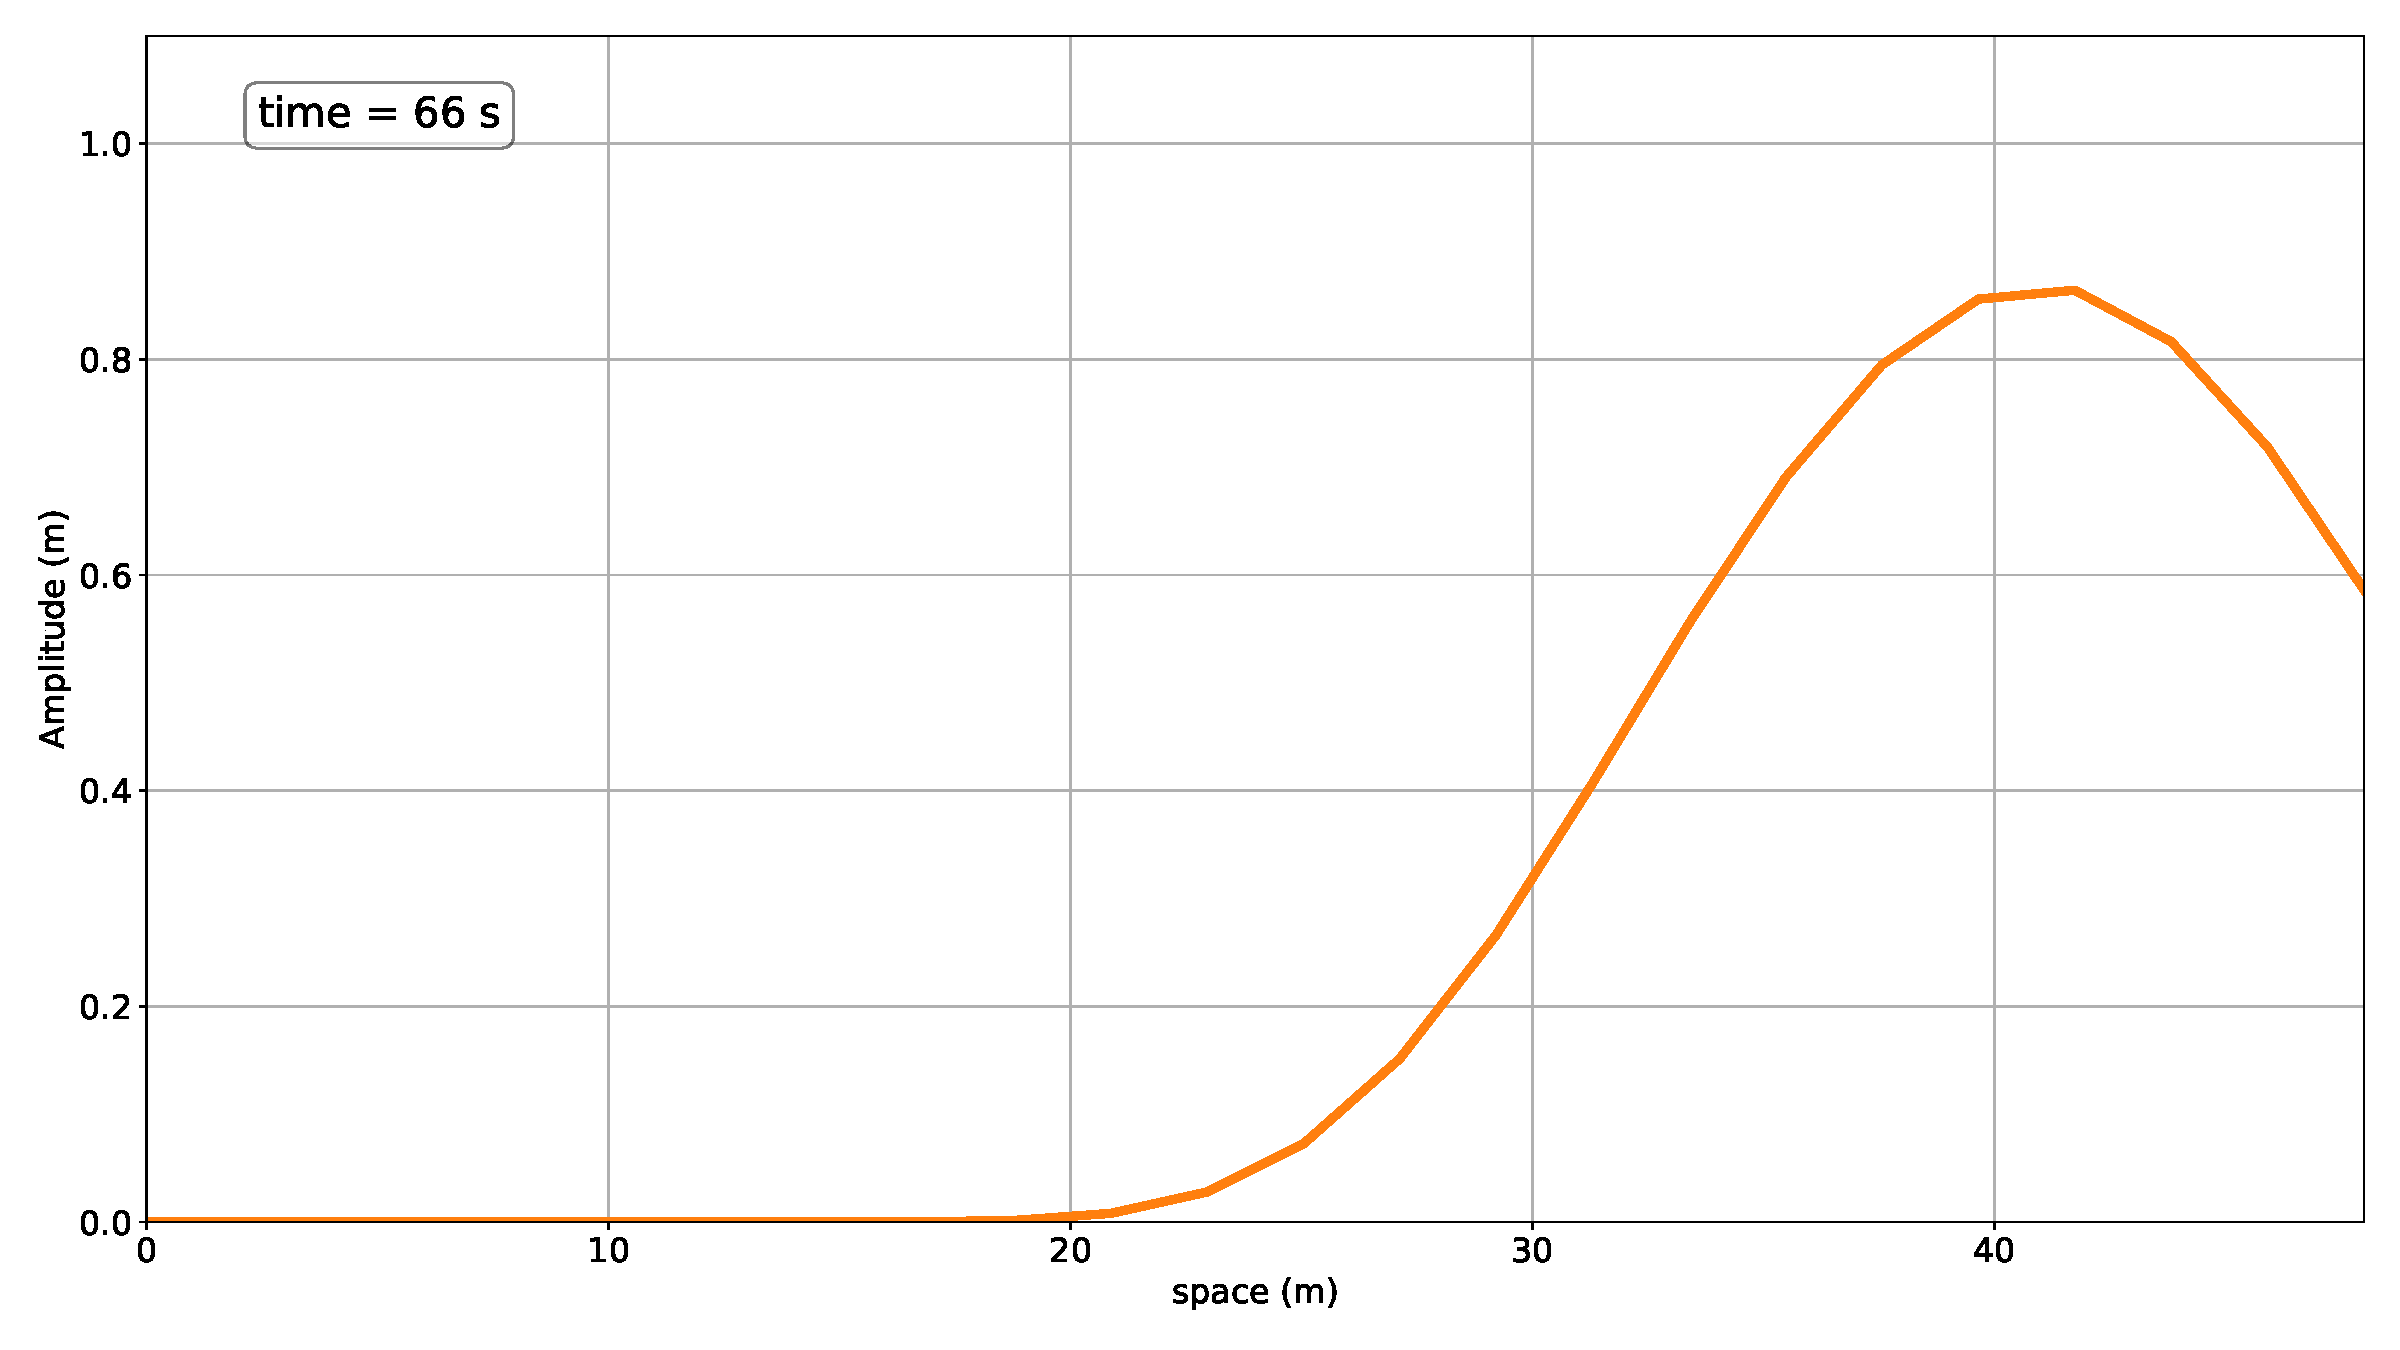
\includegraphics[width=\linewidth]{../BurgersEquation/images/Linear_Convection6.pdf}
  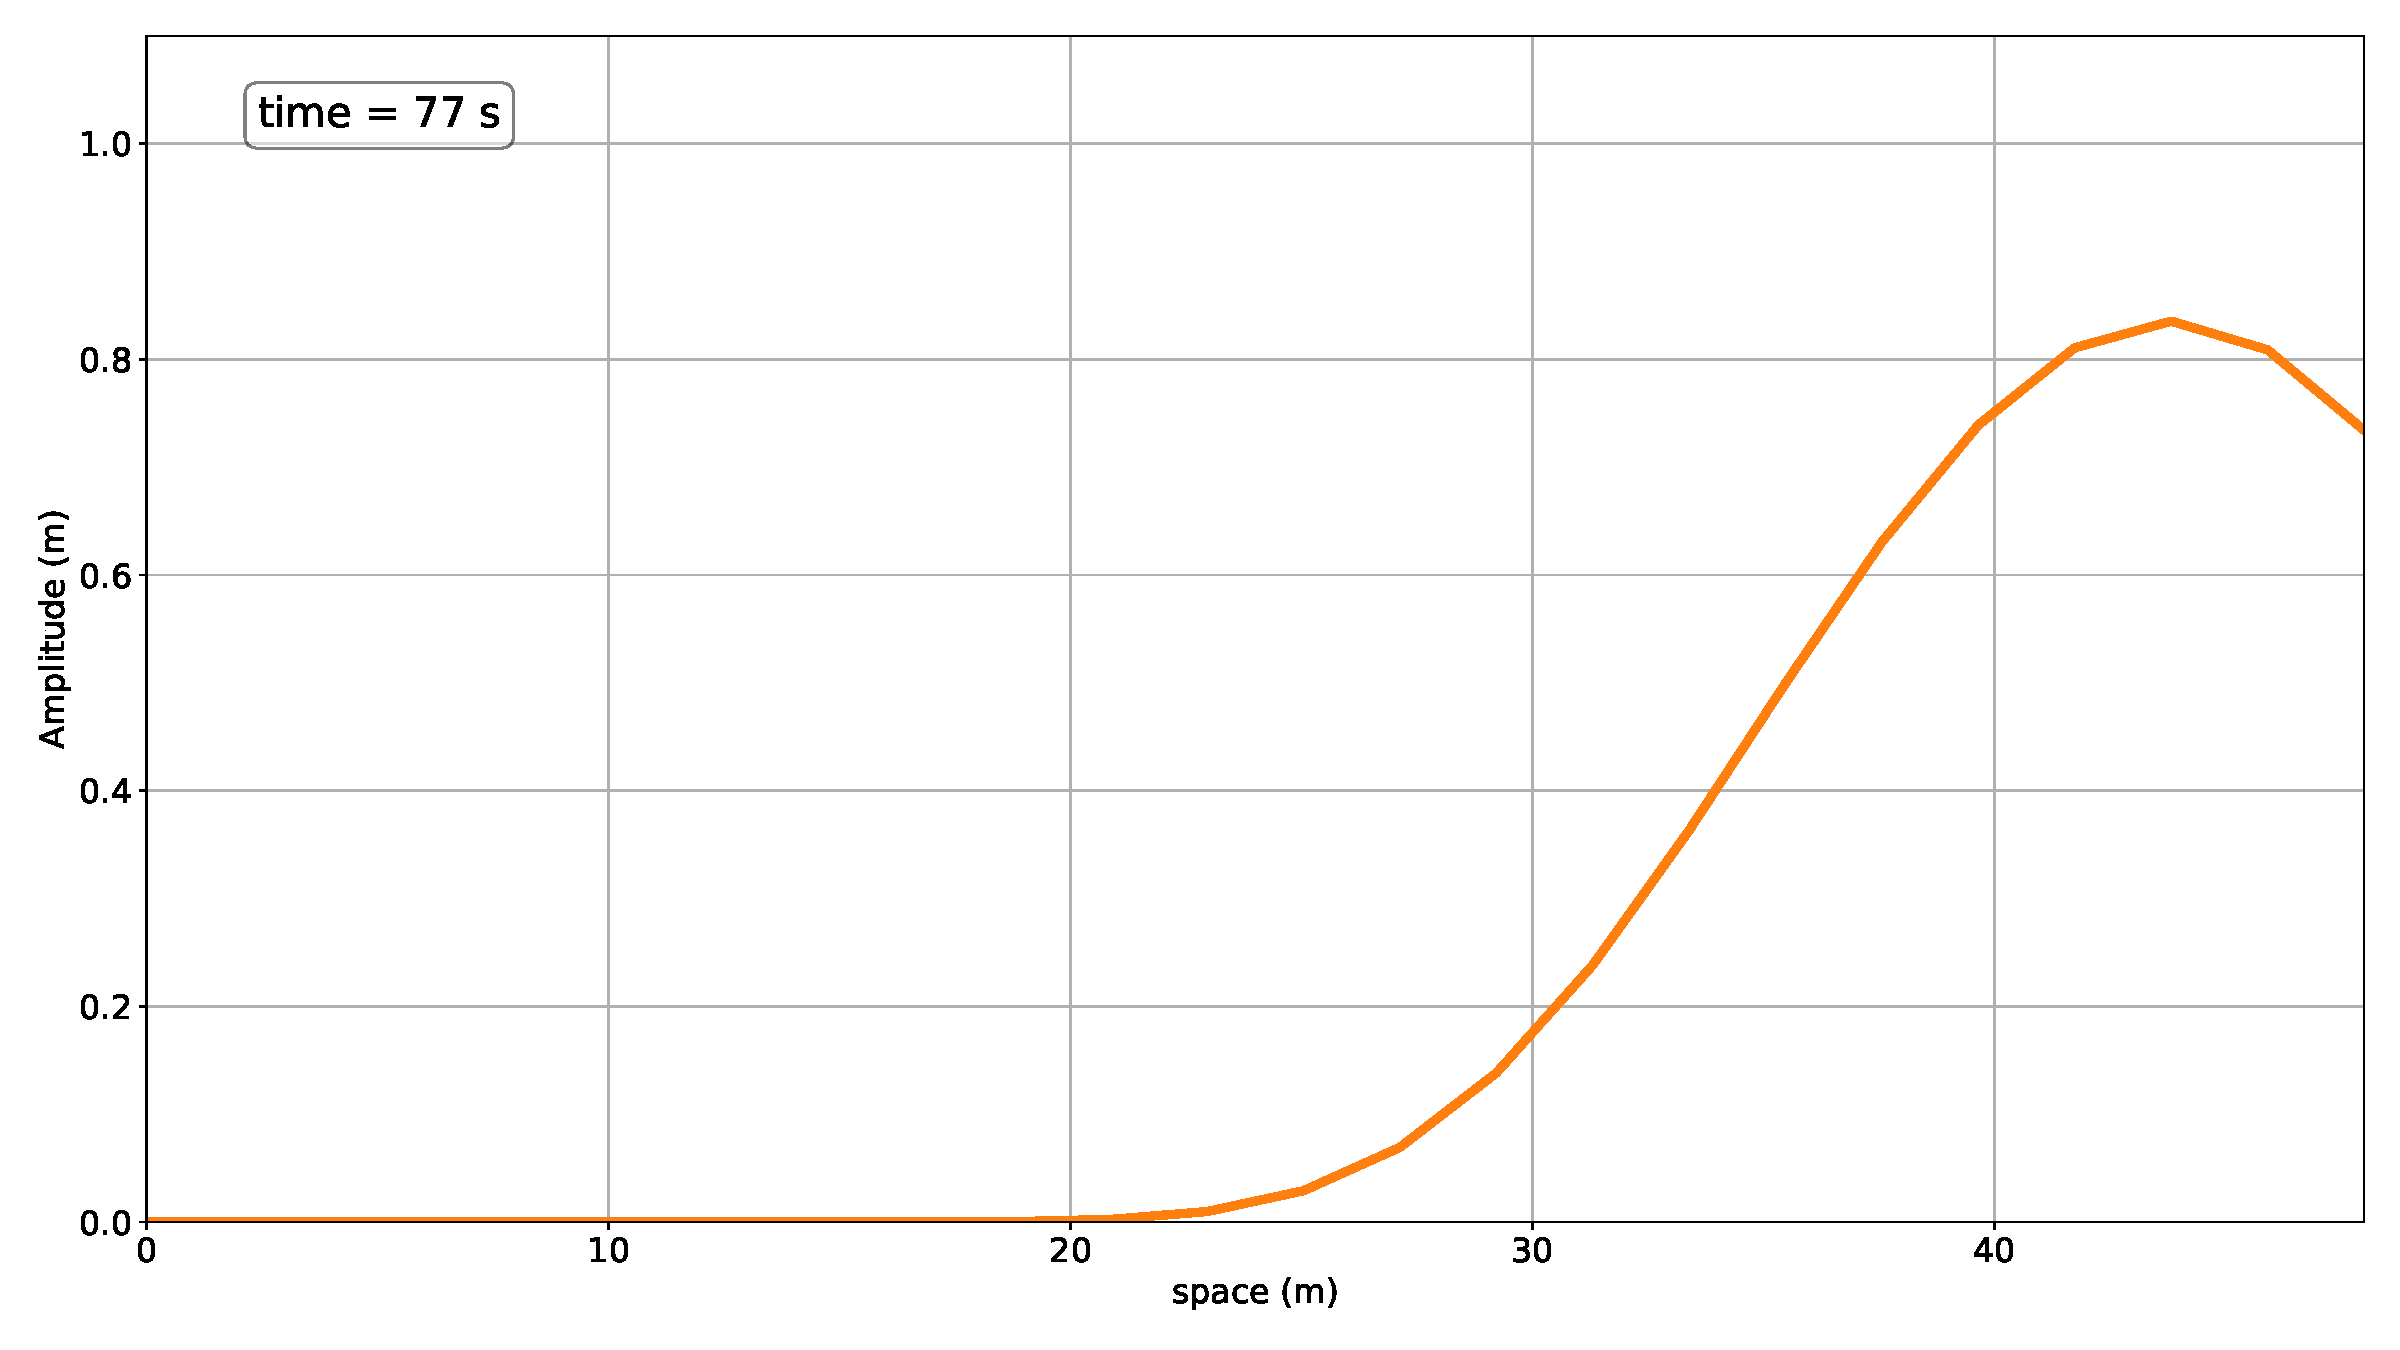
\includegraphics[width=\linewidth]{../BurgersEquation/images/Linear_Convection7.pdf}
  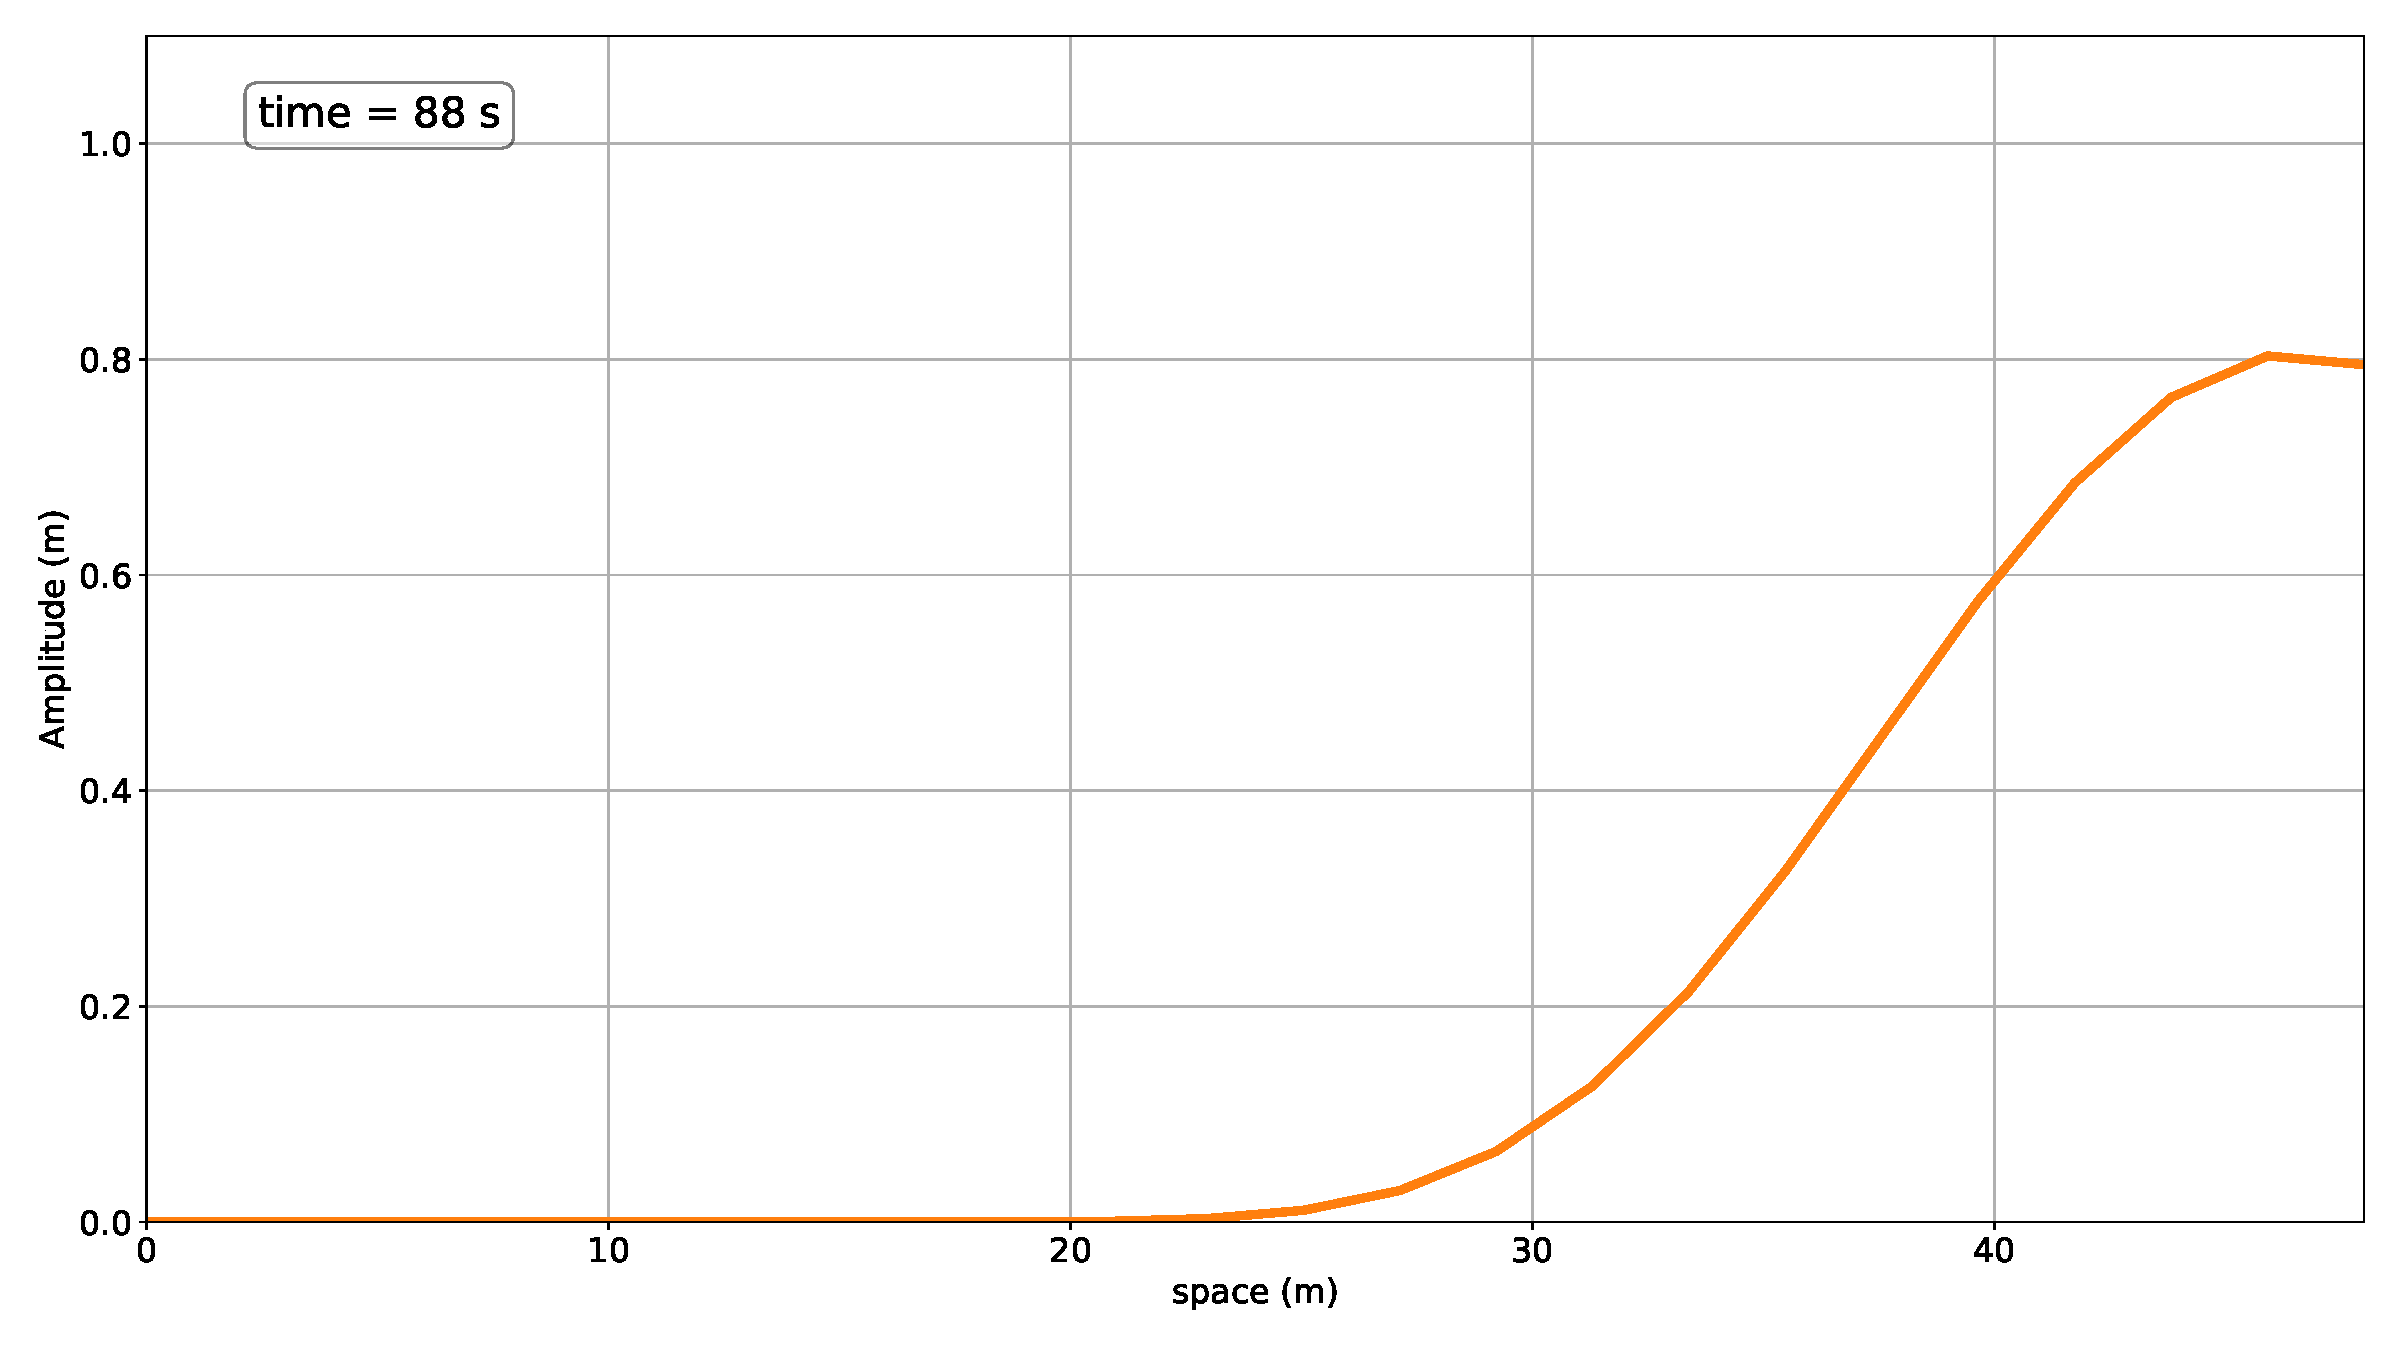
\includegraphics[width=\linewidth]{../BurgersEquation/images/Linear_Convection8.pdf}
  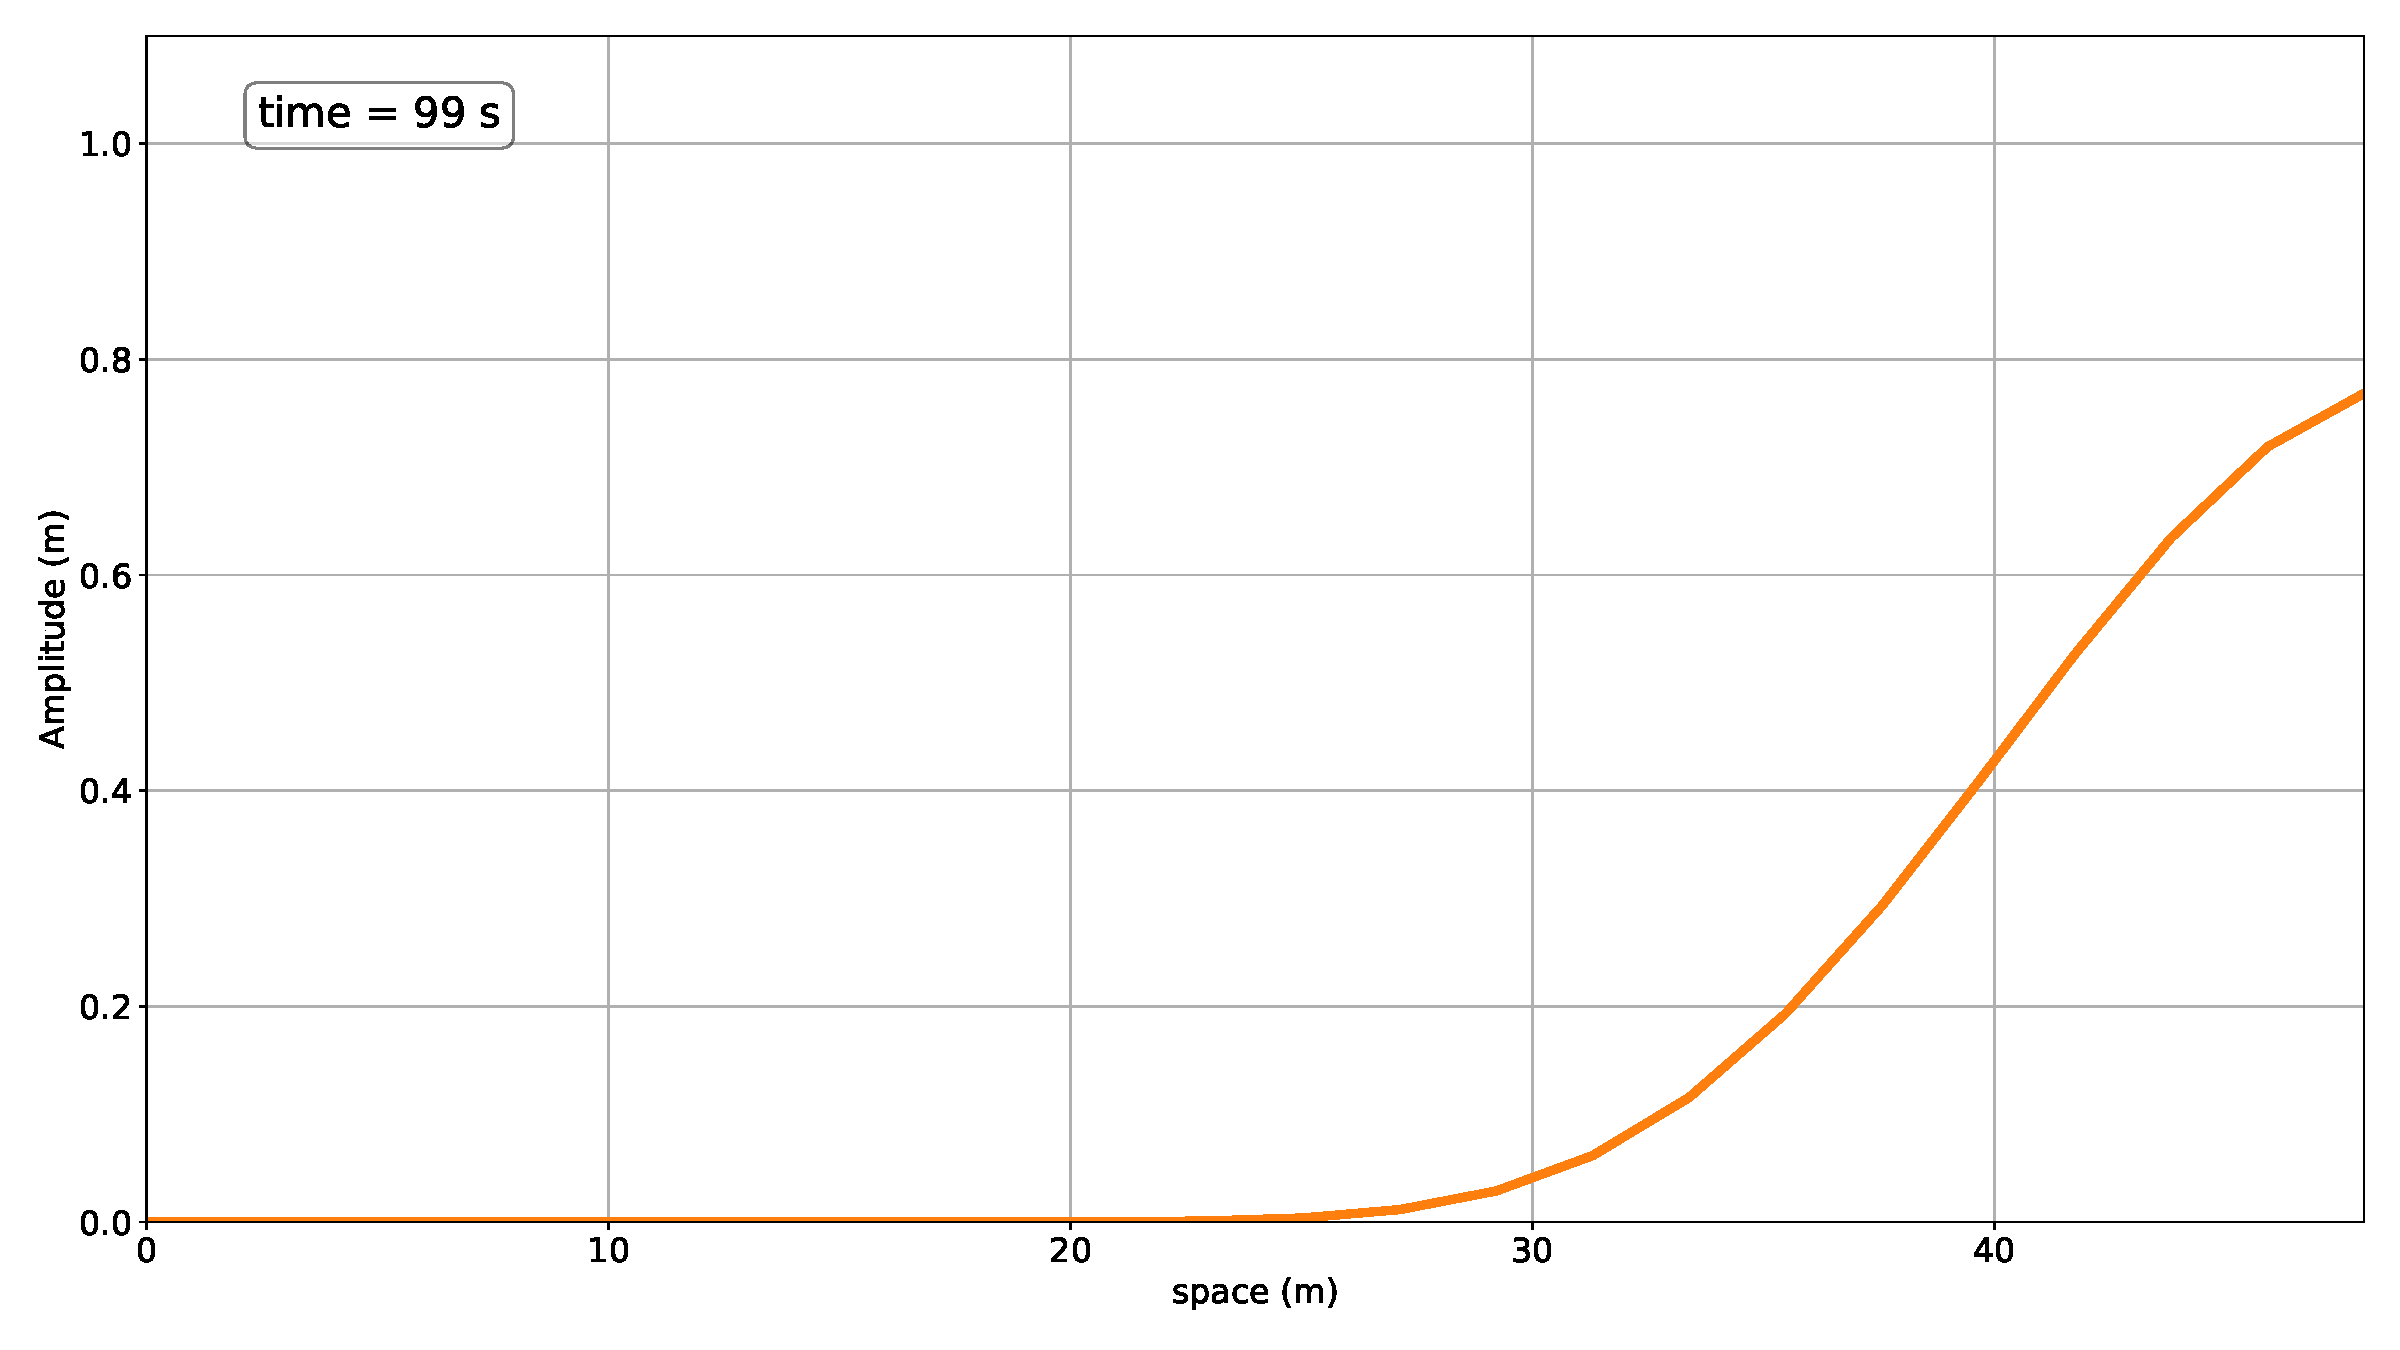
\includegraphics[width=\linewidth]{../BurgersEquation/images/Linear_Convection9.pdf}


\begin{frame}
  \frametitle{Nonlinear Convection aka. Burgers' Equation}
\begin{itemize}
  \item<1->   Viscous Burgers' equation
  \begin{itemize}
    \item $$
    \frac {\partial u}{\partial t}+u{\frac {\partial u}{\partial x}}=\nu {\frac {\partial ^{2}u}{\partial x^{2}}}
    $$
  \end{itemize}
  \item<2-> Inviscid Burgers' equation
  \begin{itemize}
    \item $$
    \frac {\partial u}{\partial t}+u{\frac {\partial u}{\partial x}}=0
    $$
  \end{itemize}
  \item<3-> Appears in
  \begin{itemize}
    \item Fluid dynamics
    \item Nonlinear acoustics
    \item Traffic flow
  \end{itemize}
\end{itemize}
\end{frame}

% \begin{frame}
%   \frametitle{Nonlinear Convection aka. Burgers' Equation}
%   \begin{center}
%     \includemedia[width=1\linewidth,height=.5\linewidth,activate=pageopen,
%   passcontext,
%   transparent,
%   addresource=slides/images/Linear_Convection.mp4,
%   flashvars={source=slides/images/Linear_Convection.mp4}
%   ]{\includegraphics[width=\linewidth]{slides/images/Nonlinear_Convection_thumb.pdf}}{VPlayer.swf}
%   \end{center}
% \end{frame}


% 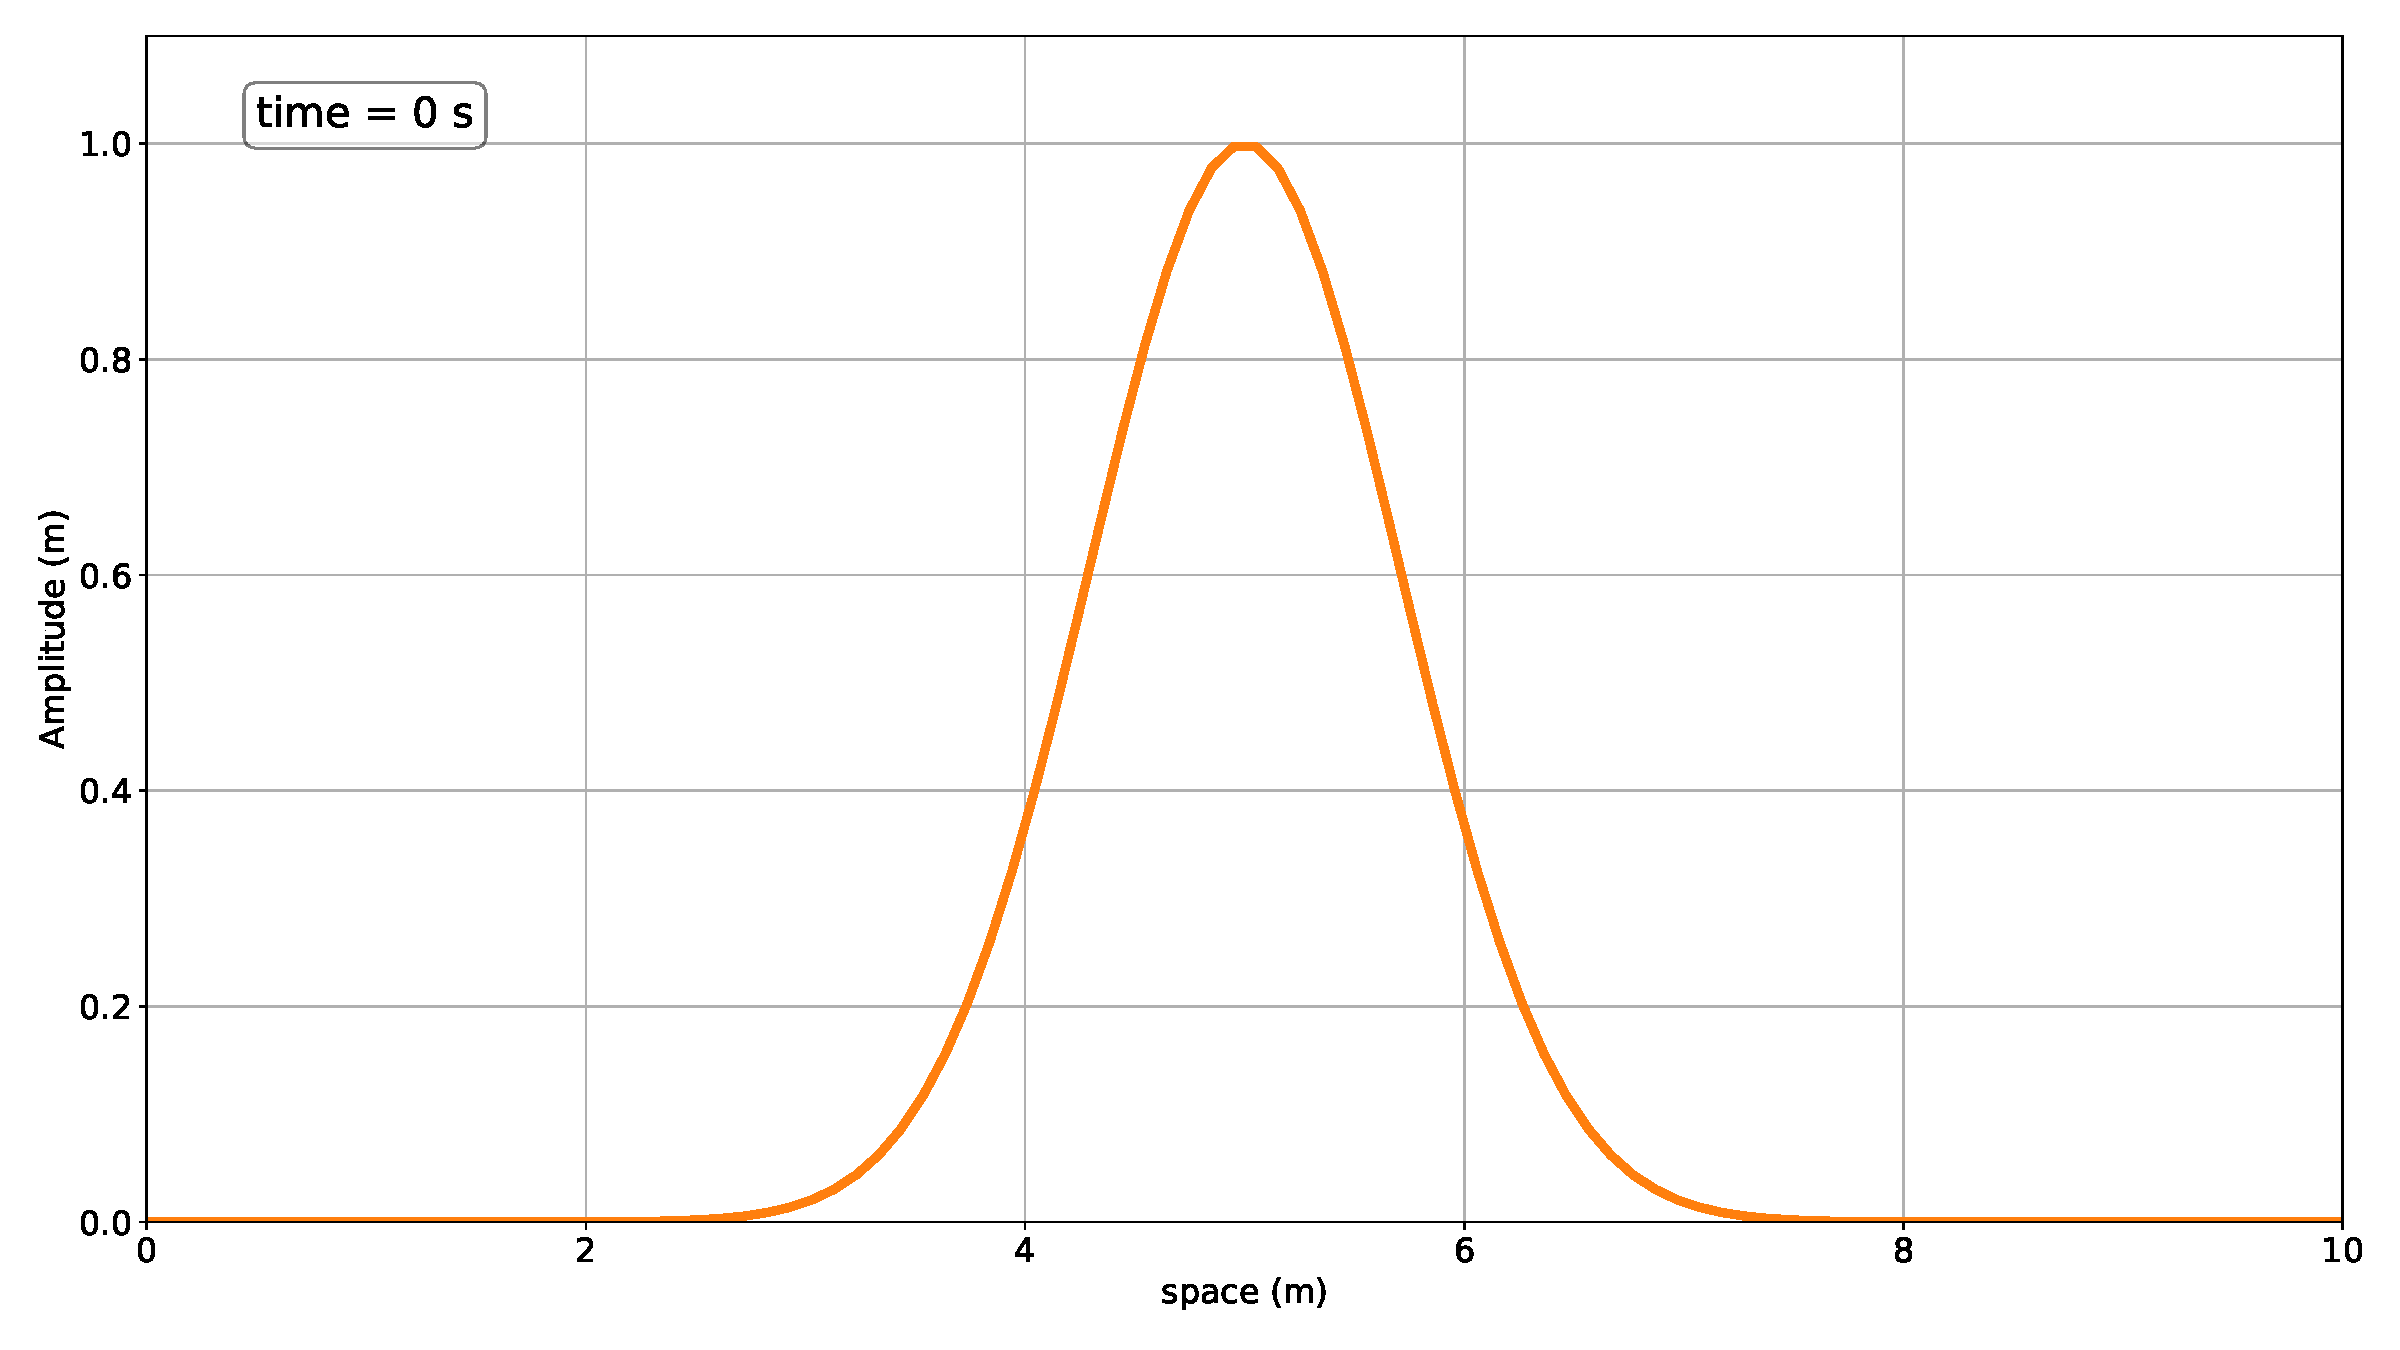
\includegraphics[width=\linewidth]{../BurgersEquation/images/Nonlinear_Convection0.pdf}
% 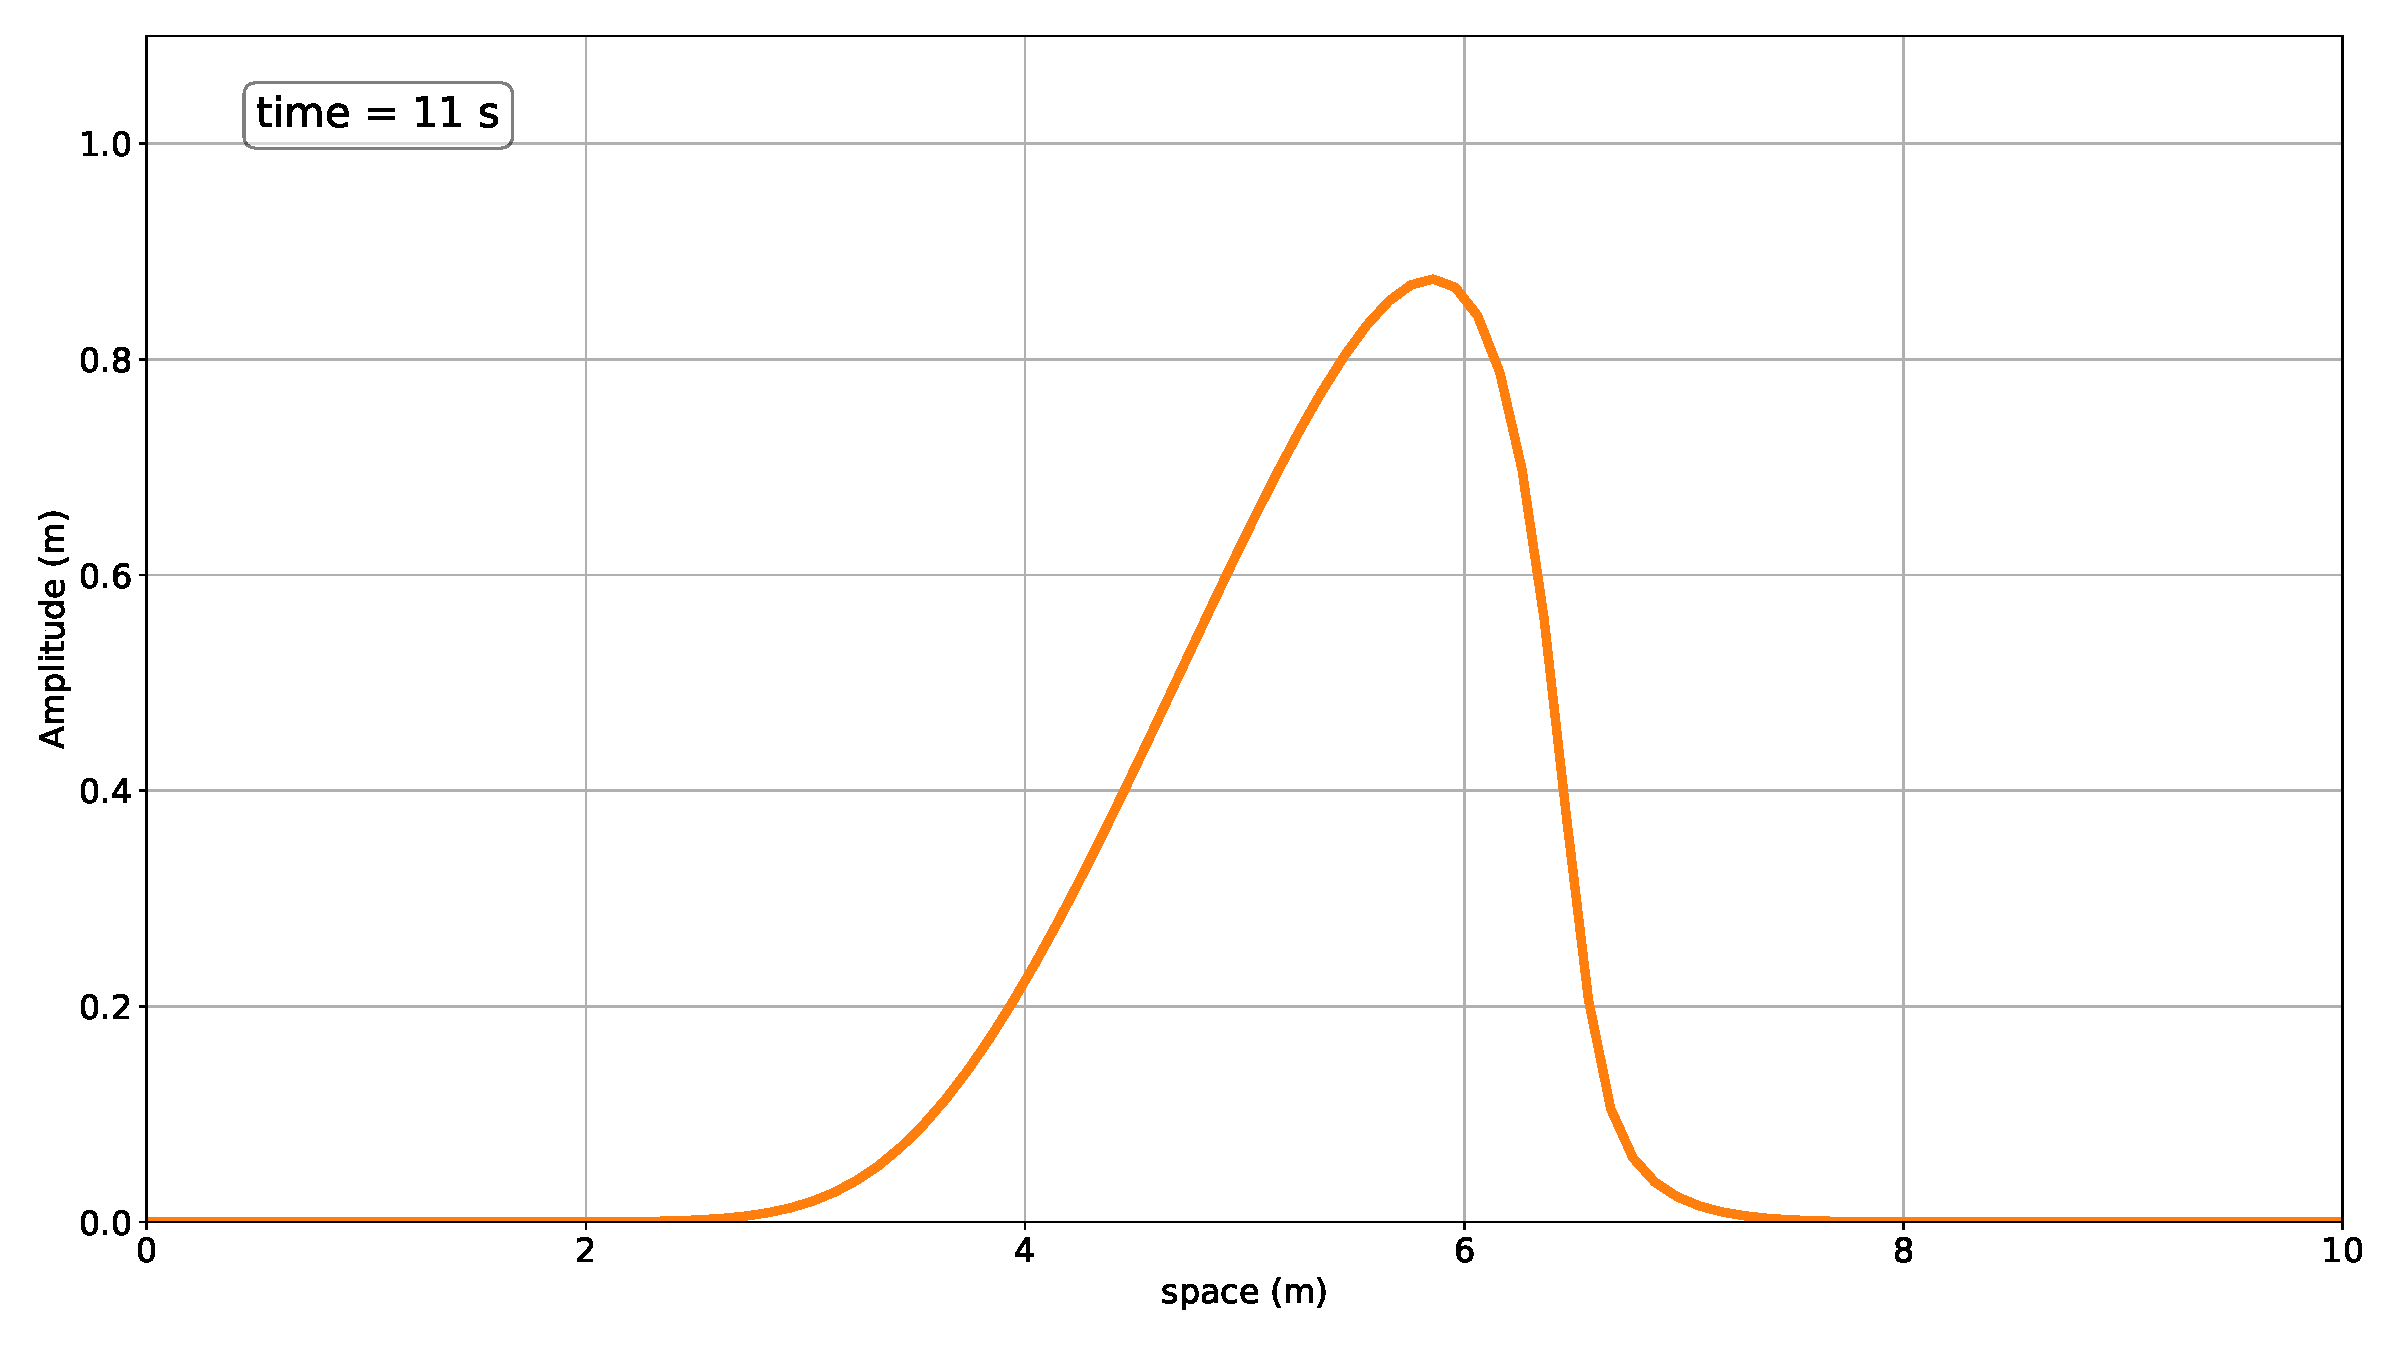
\includegraphics[width=\linewidth]{../BurgersEquation/images/Nonlinear_Convection1.pdf}
% 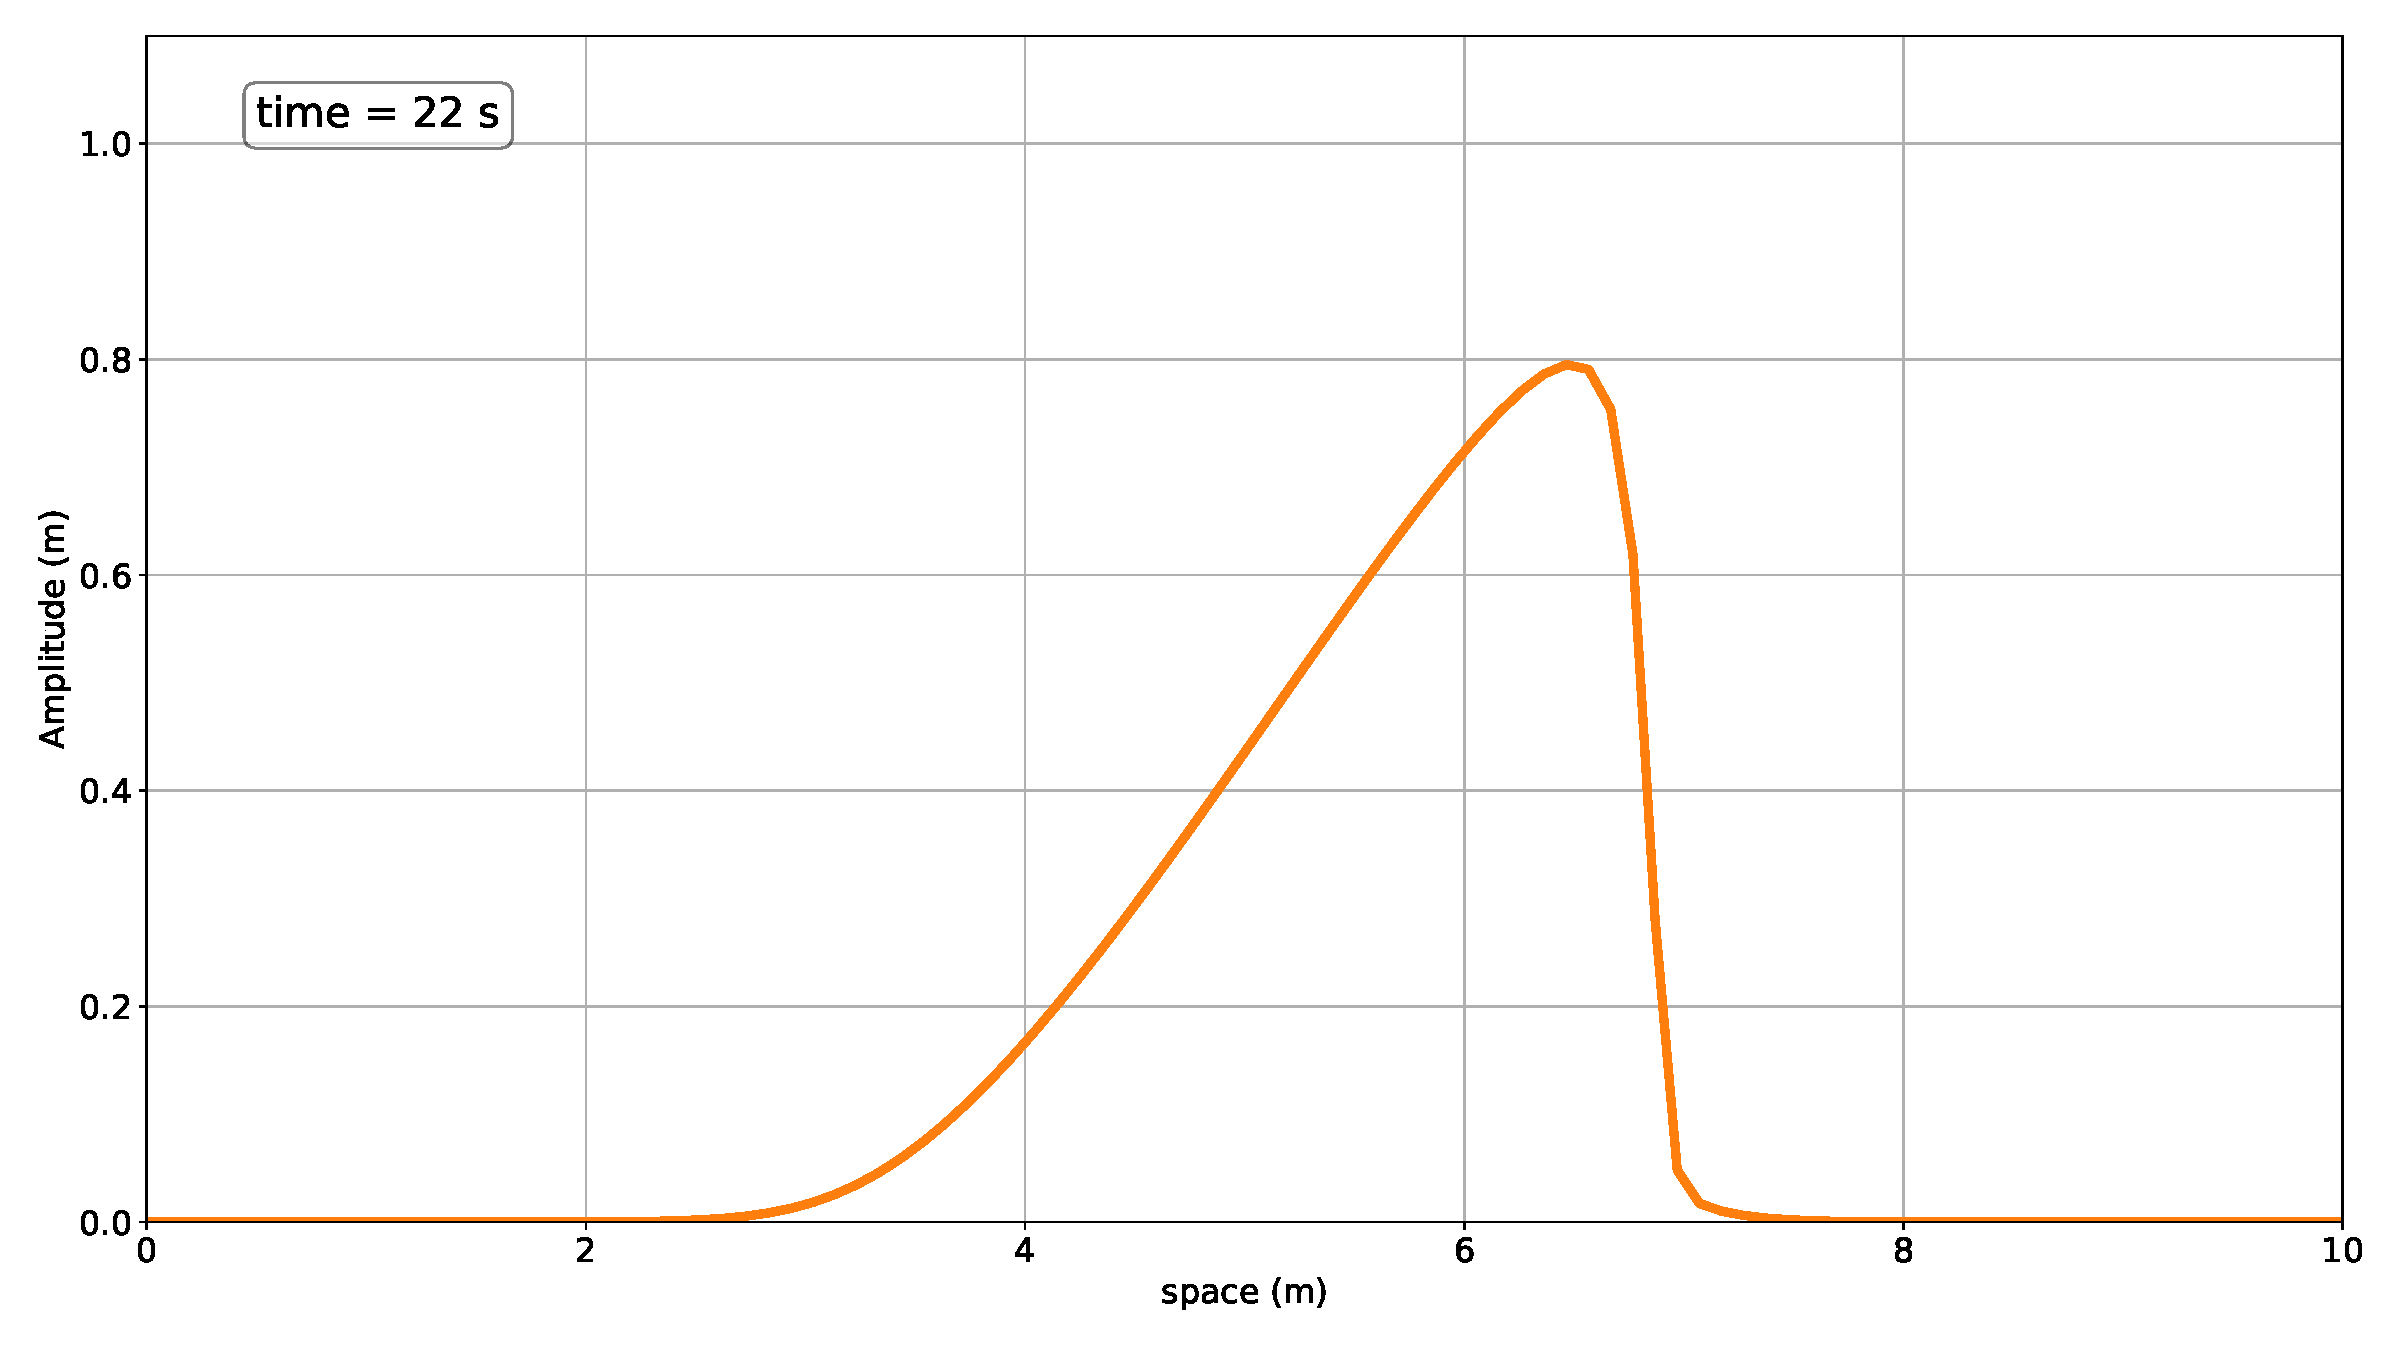
\includegraphics[width=\linewidth]{../BurgersEquation/images/Nonlinear_Convection2.pdf}
% 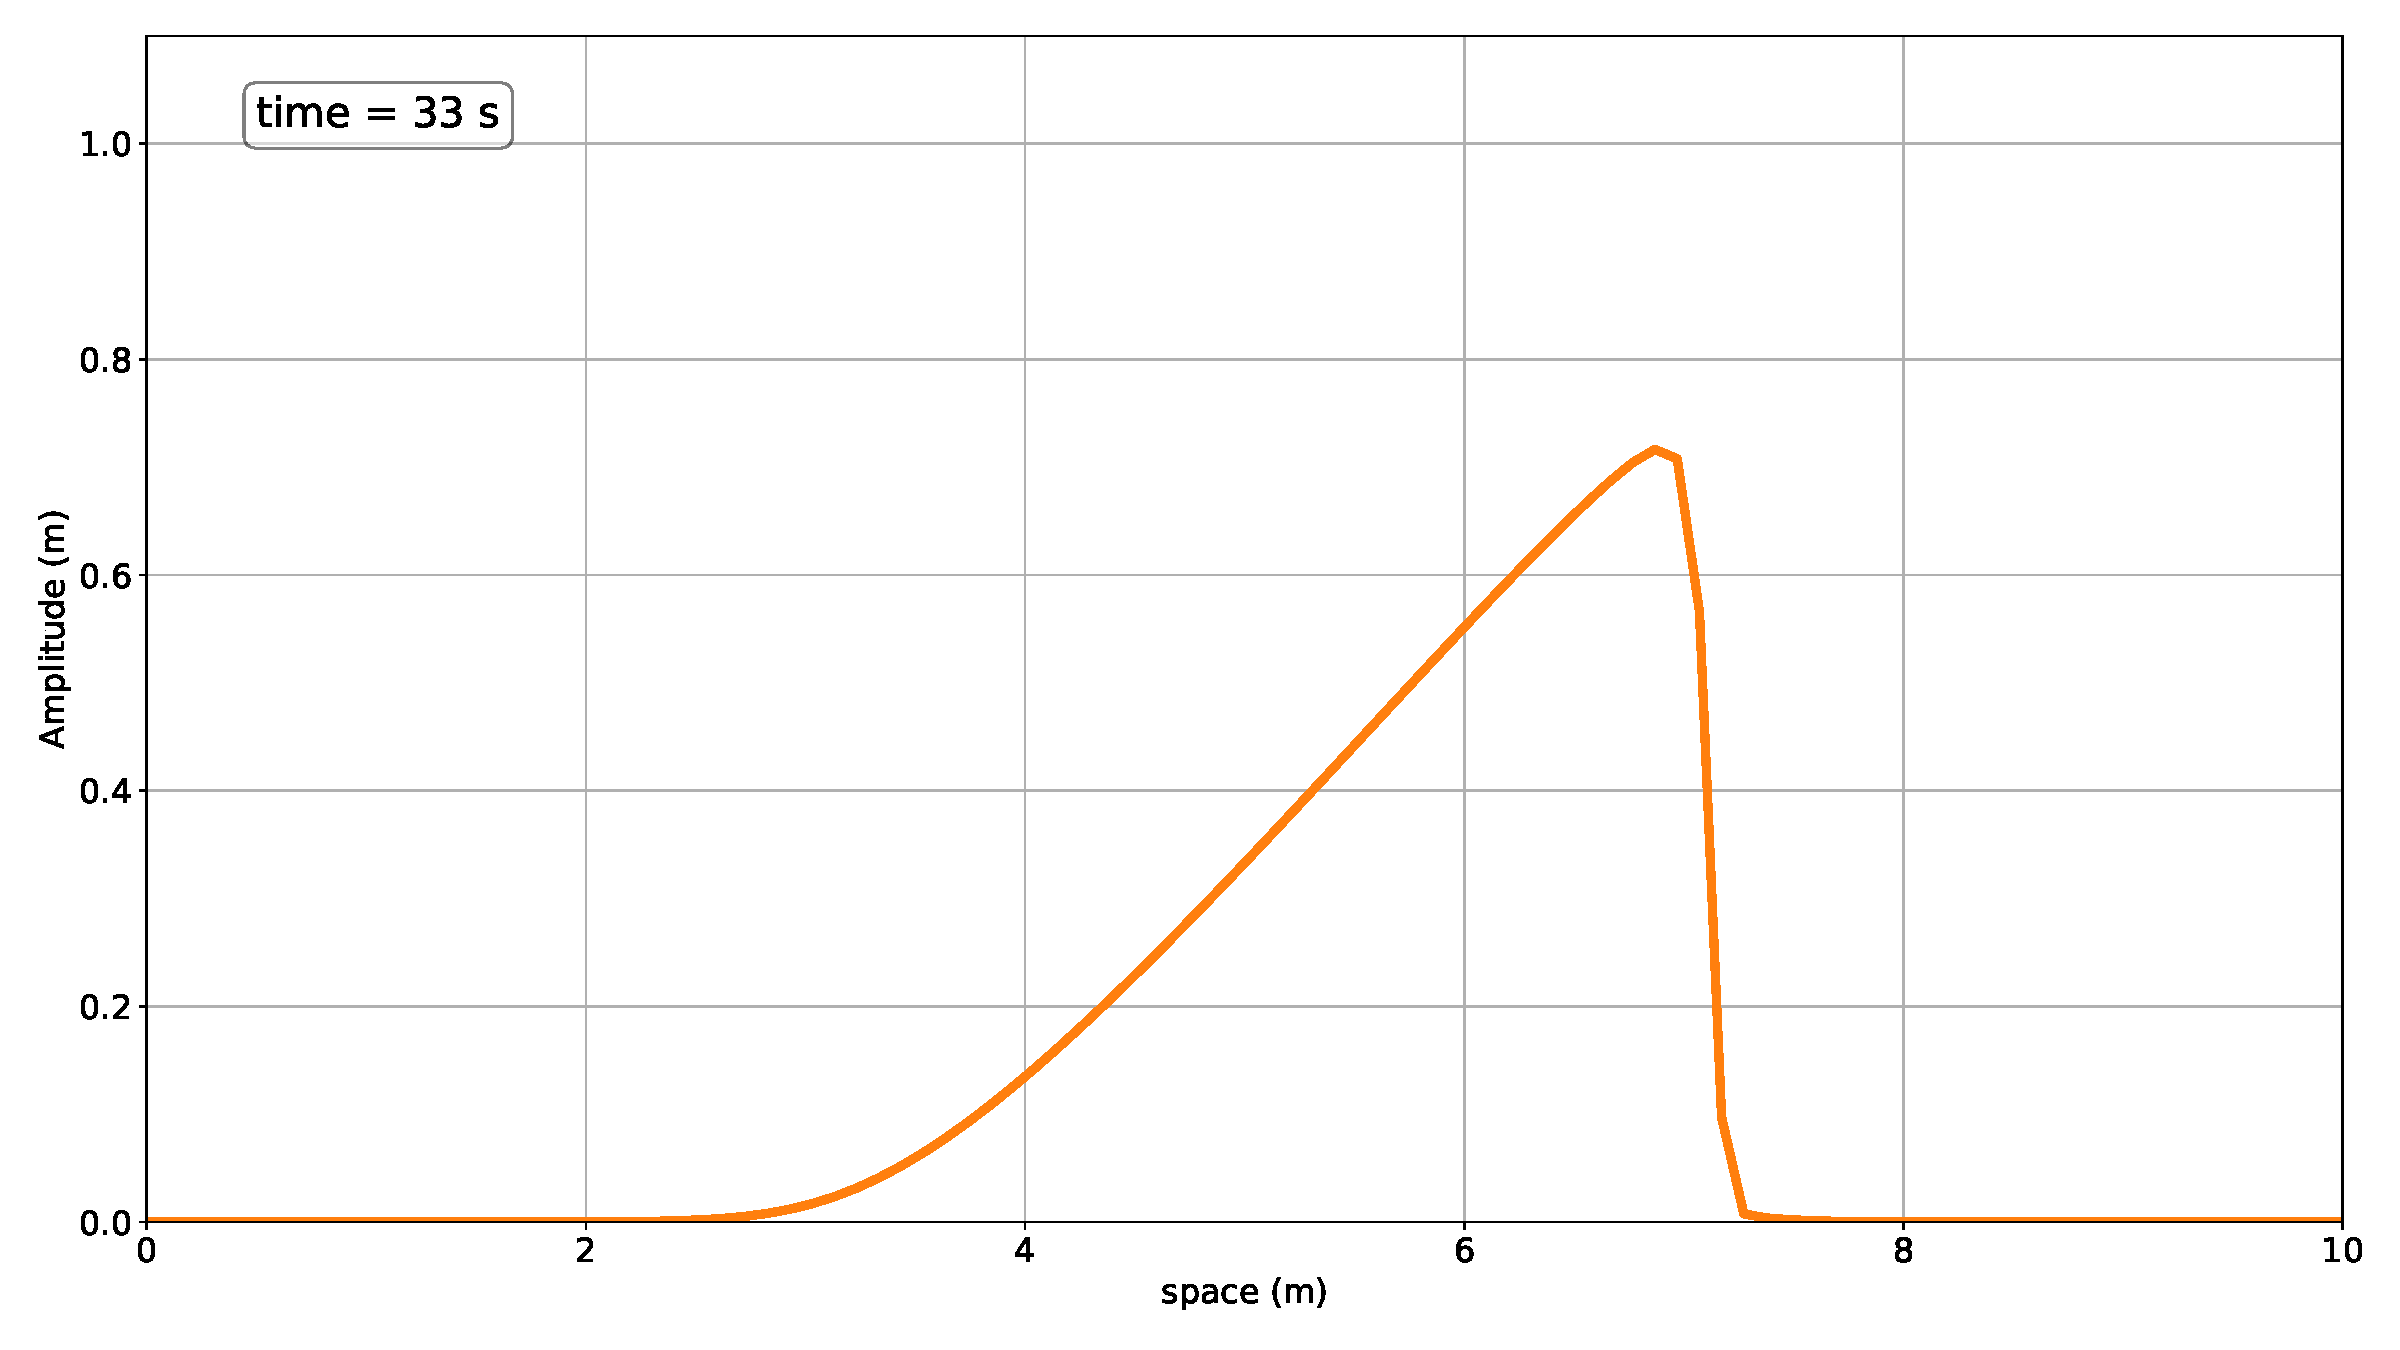
\includegraphics[width=\linewidth]{../BurgersEquation/images/Nonlinear_Convection3.pdf}
% 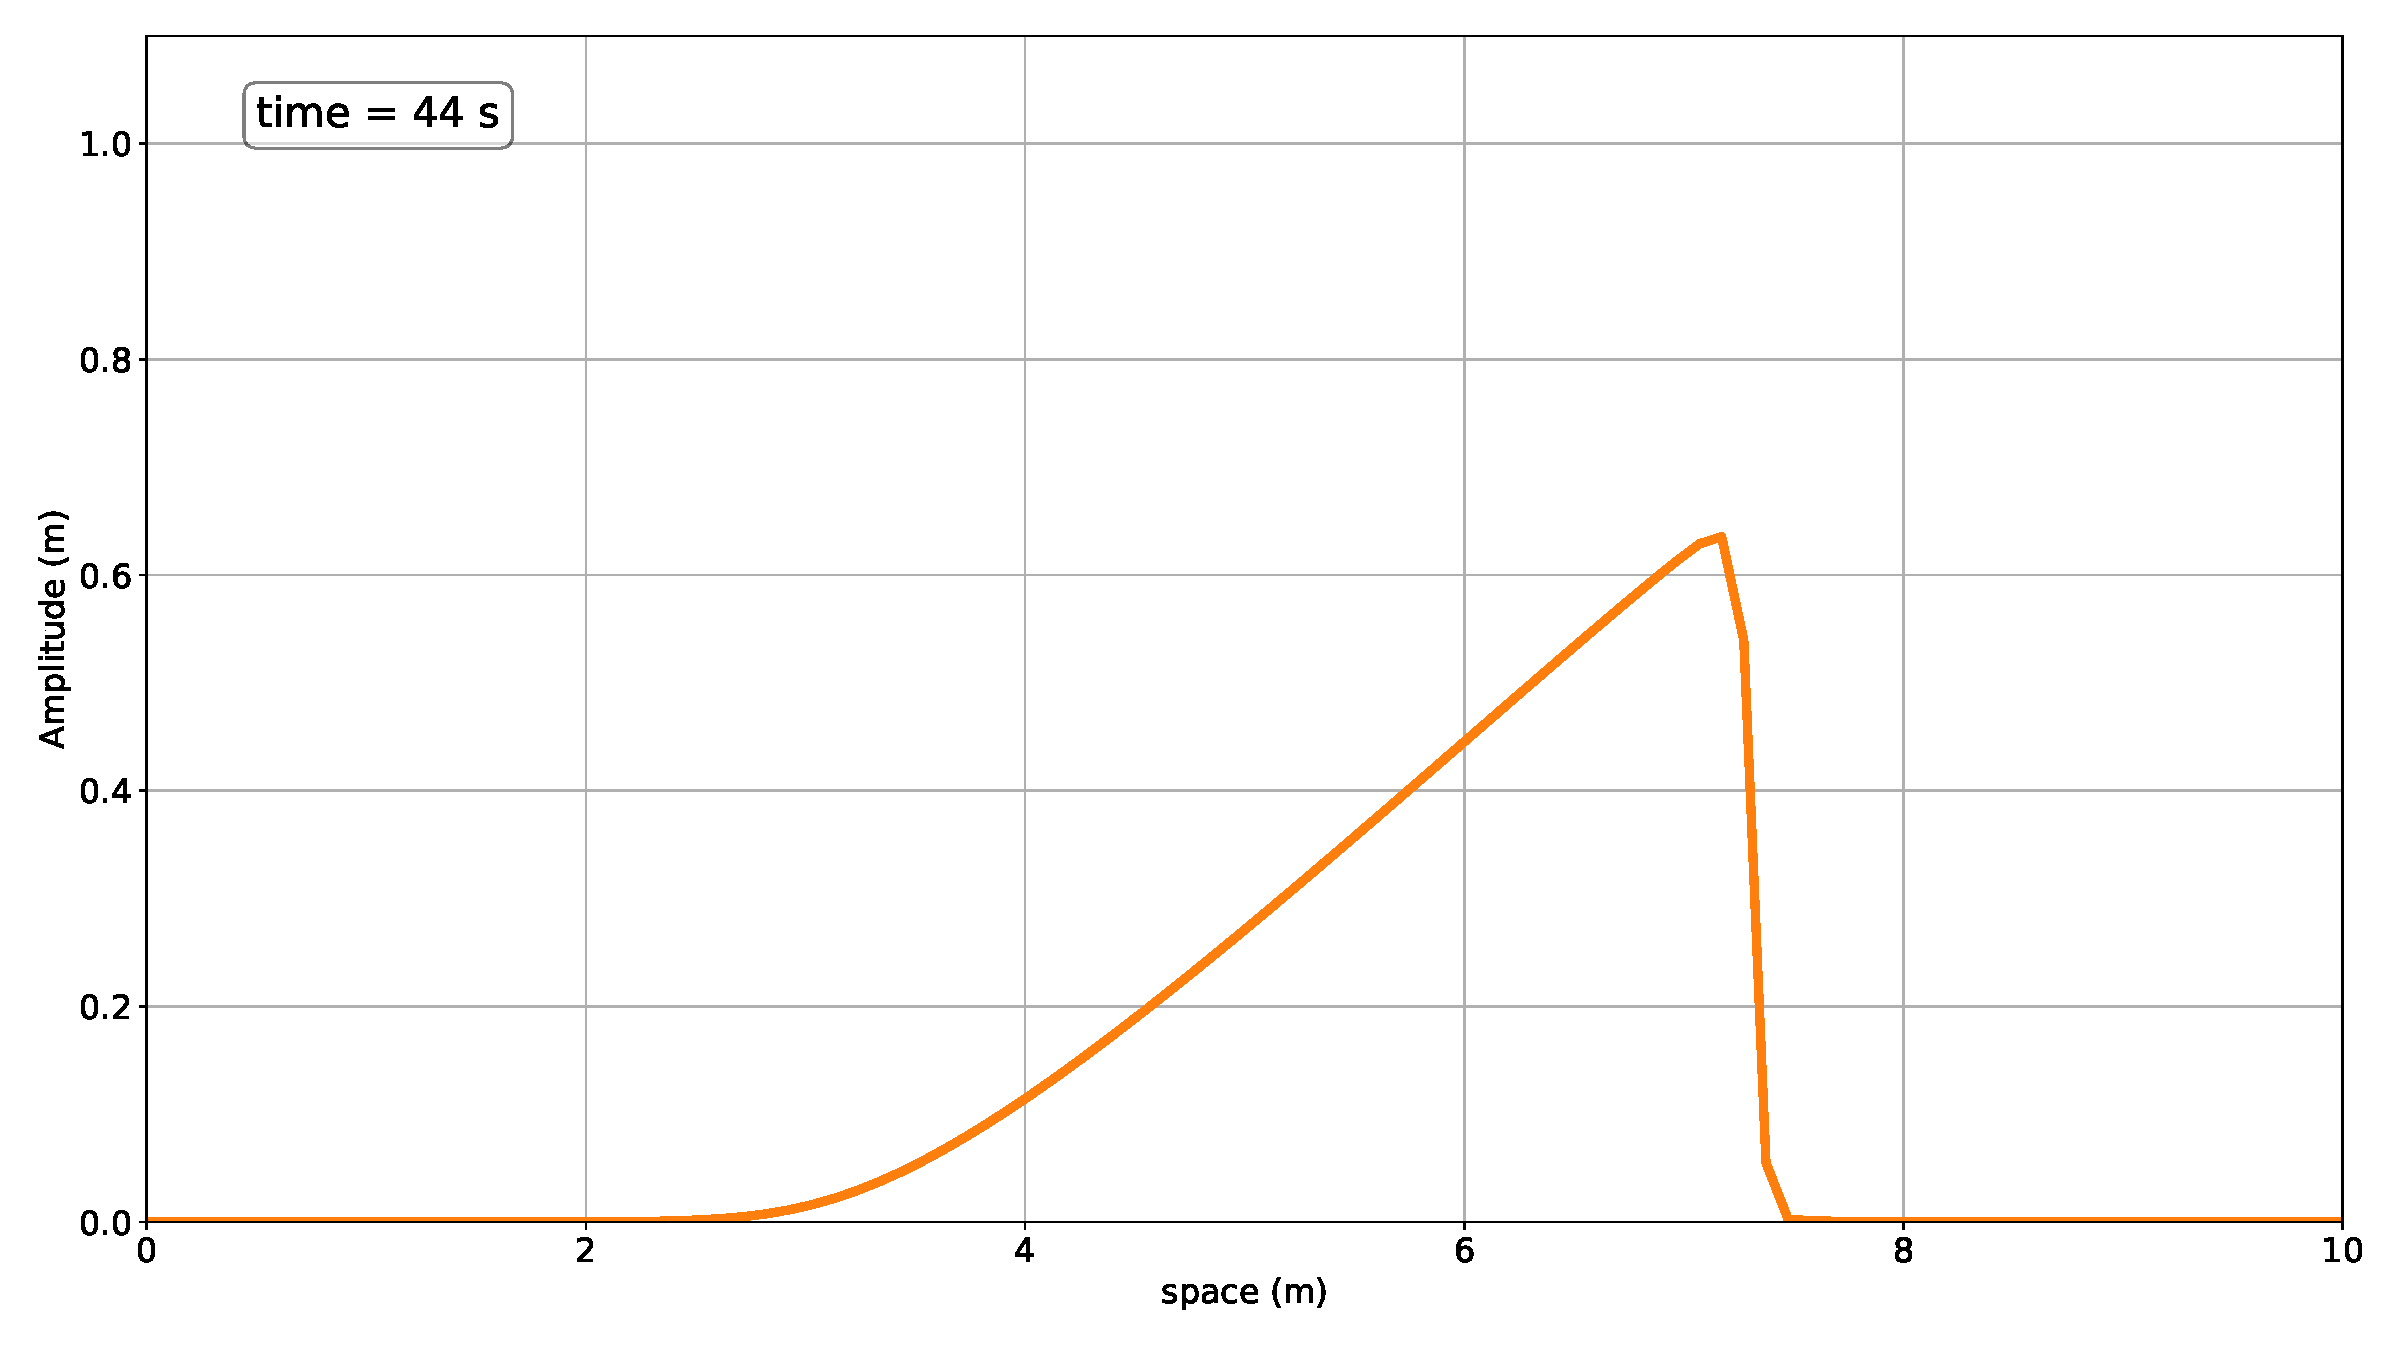
\includegraphics[width=\linewidth]{../BurgersEquation/images/Nonlinear_Convection4.pdf}
% 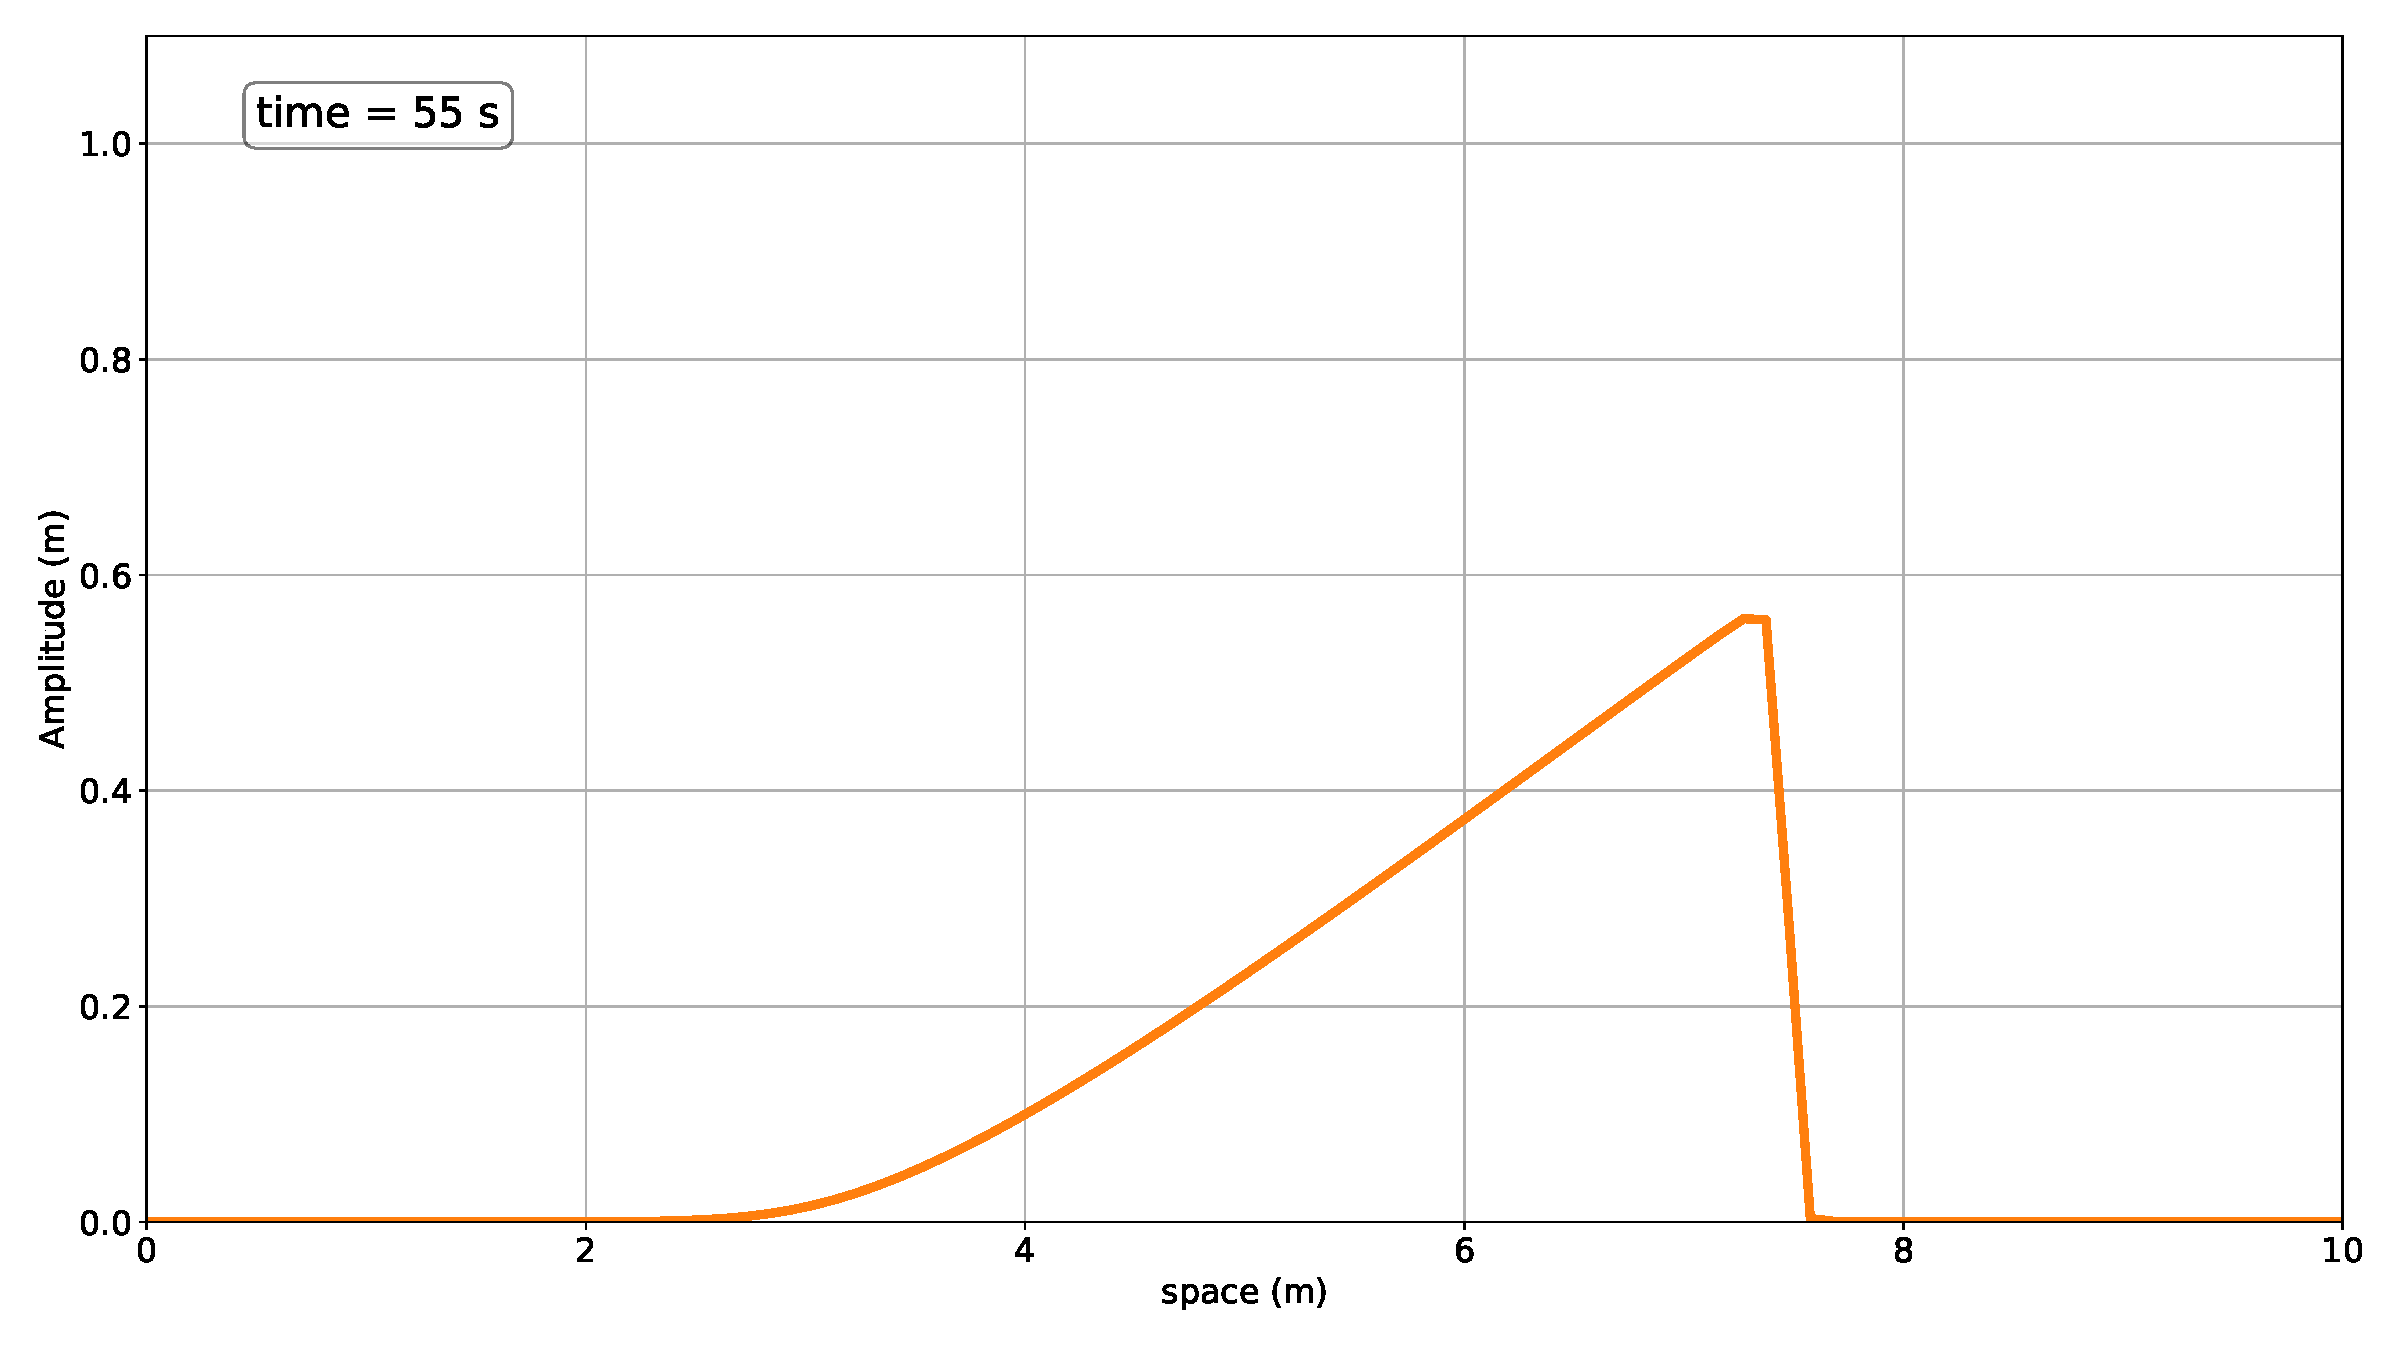
\includegraphics[width=\linewidth]{../BurgersEquation/images/Nonlinear_Convection5.pdf}
% 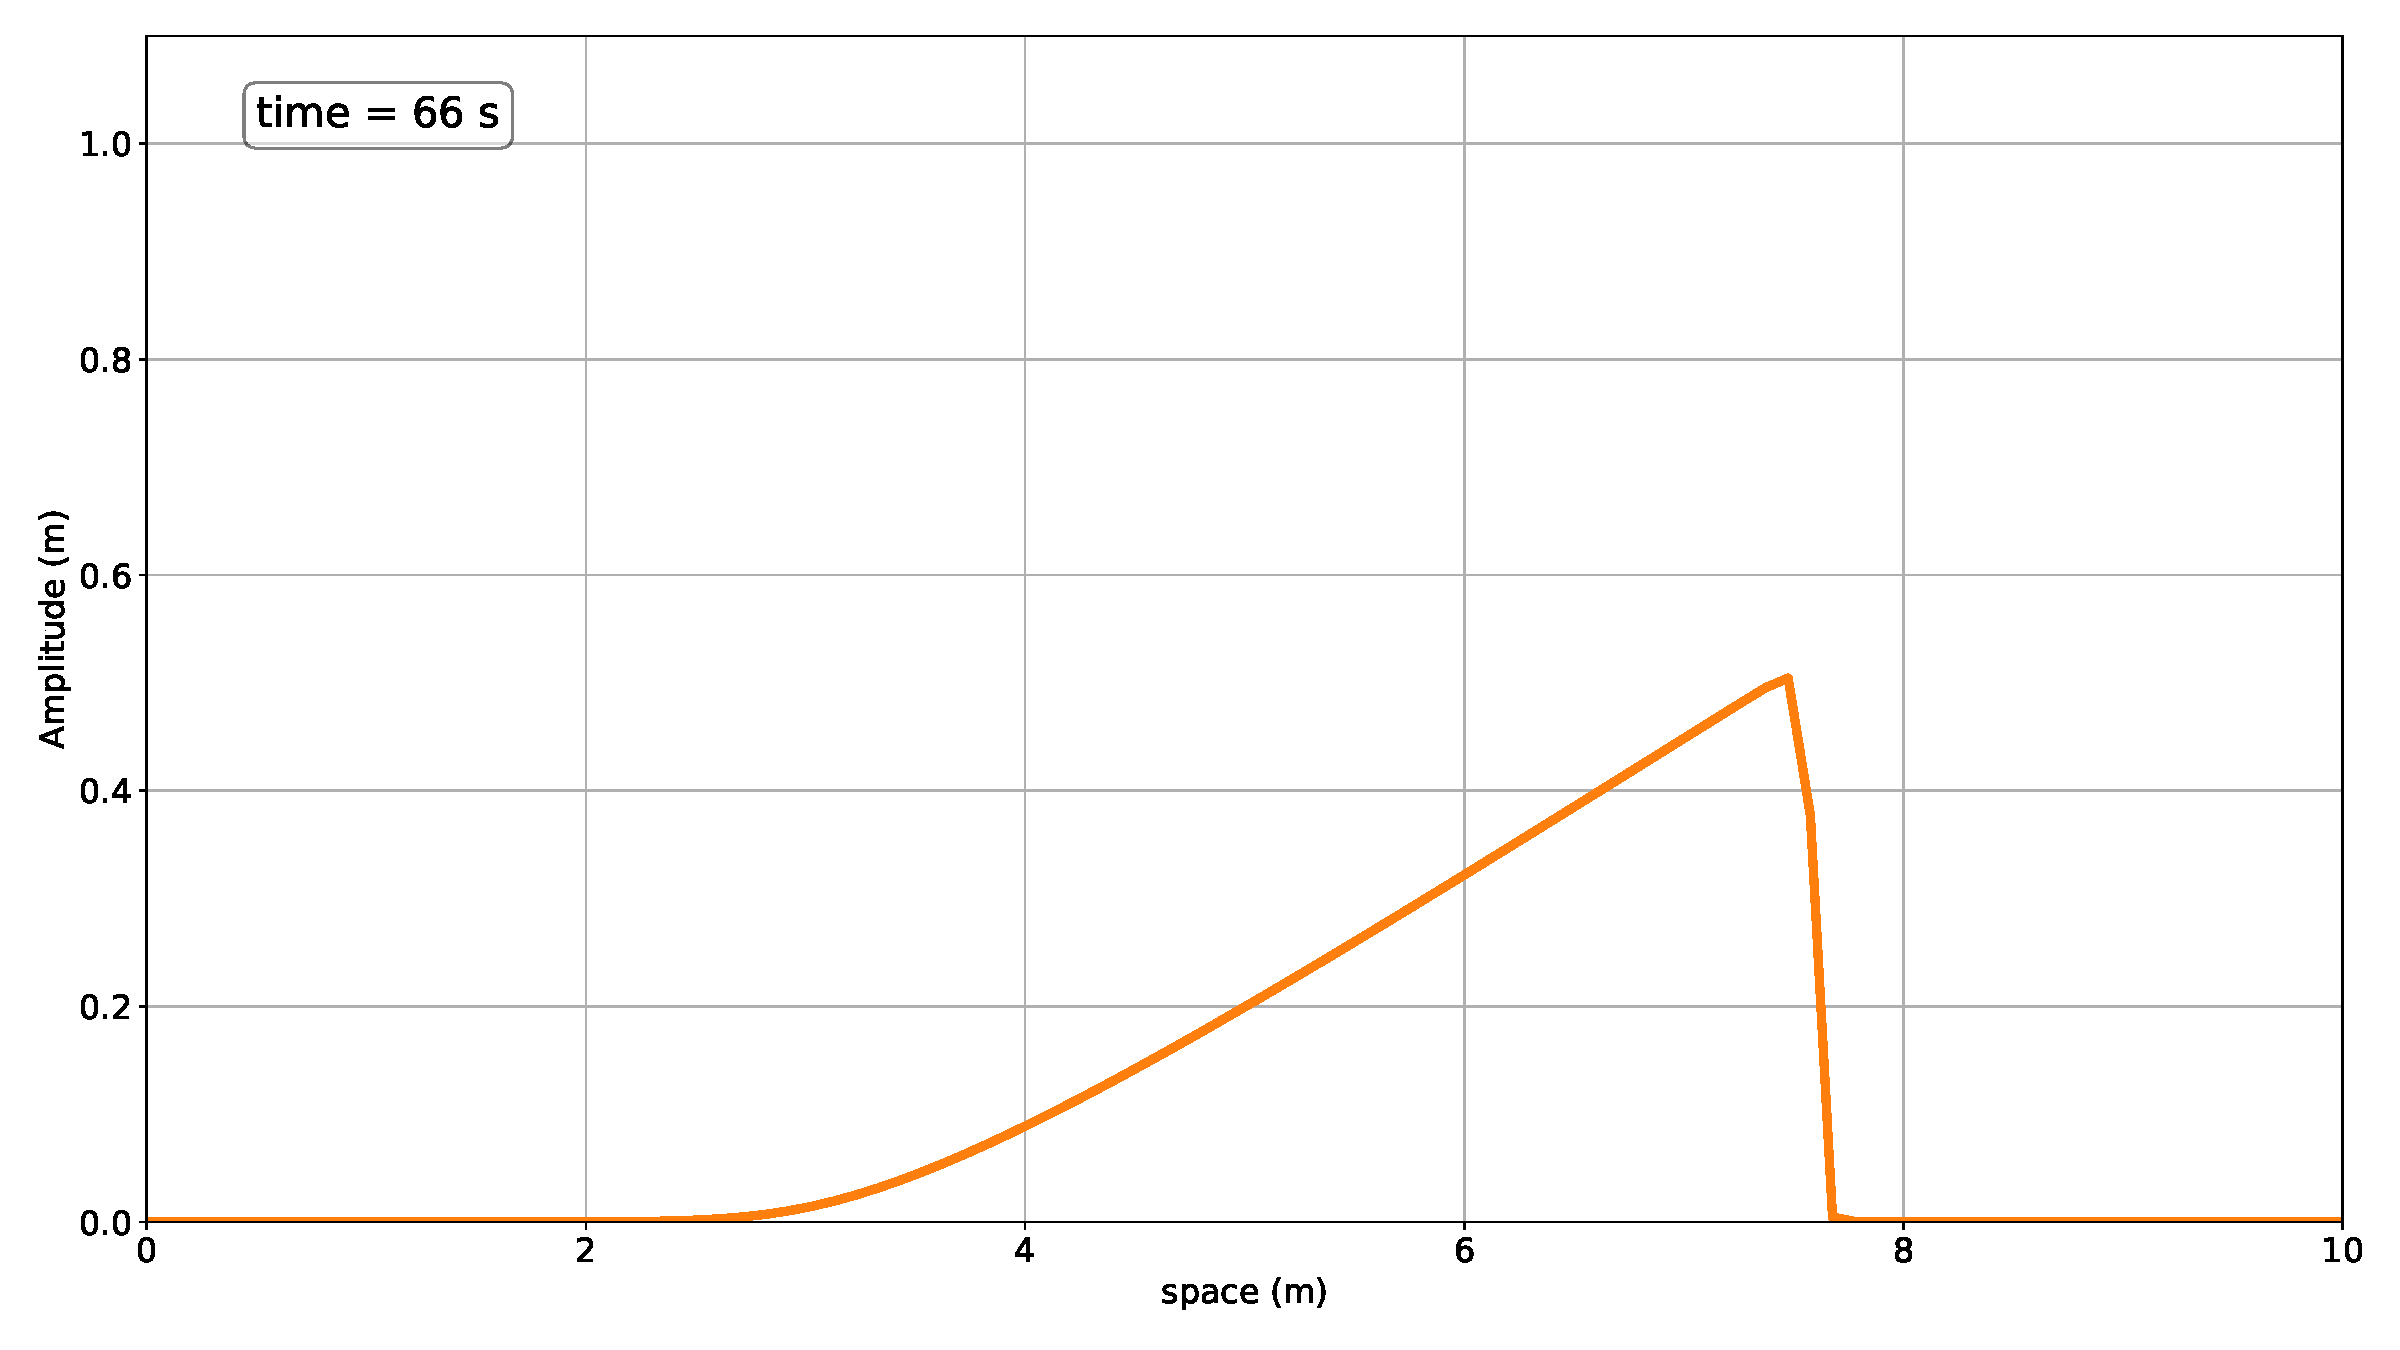
\includegraphics[width=\linewidth]{../BurgersEquation/images/Nonlinear_Convection6.pdf}
% 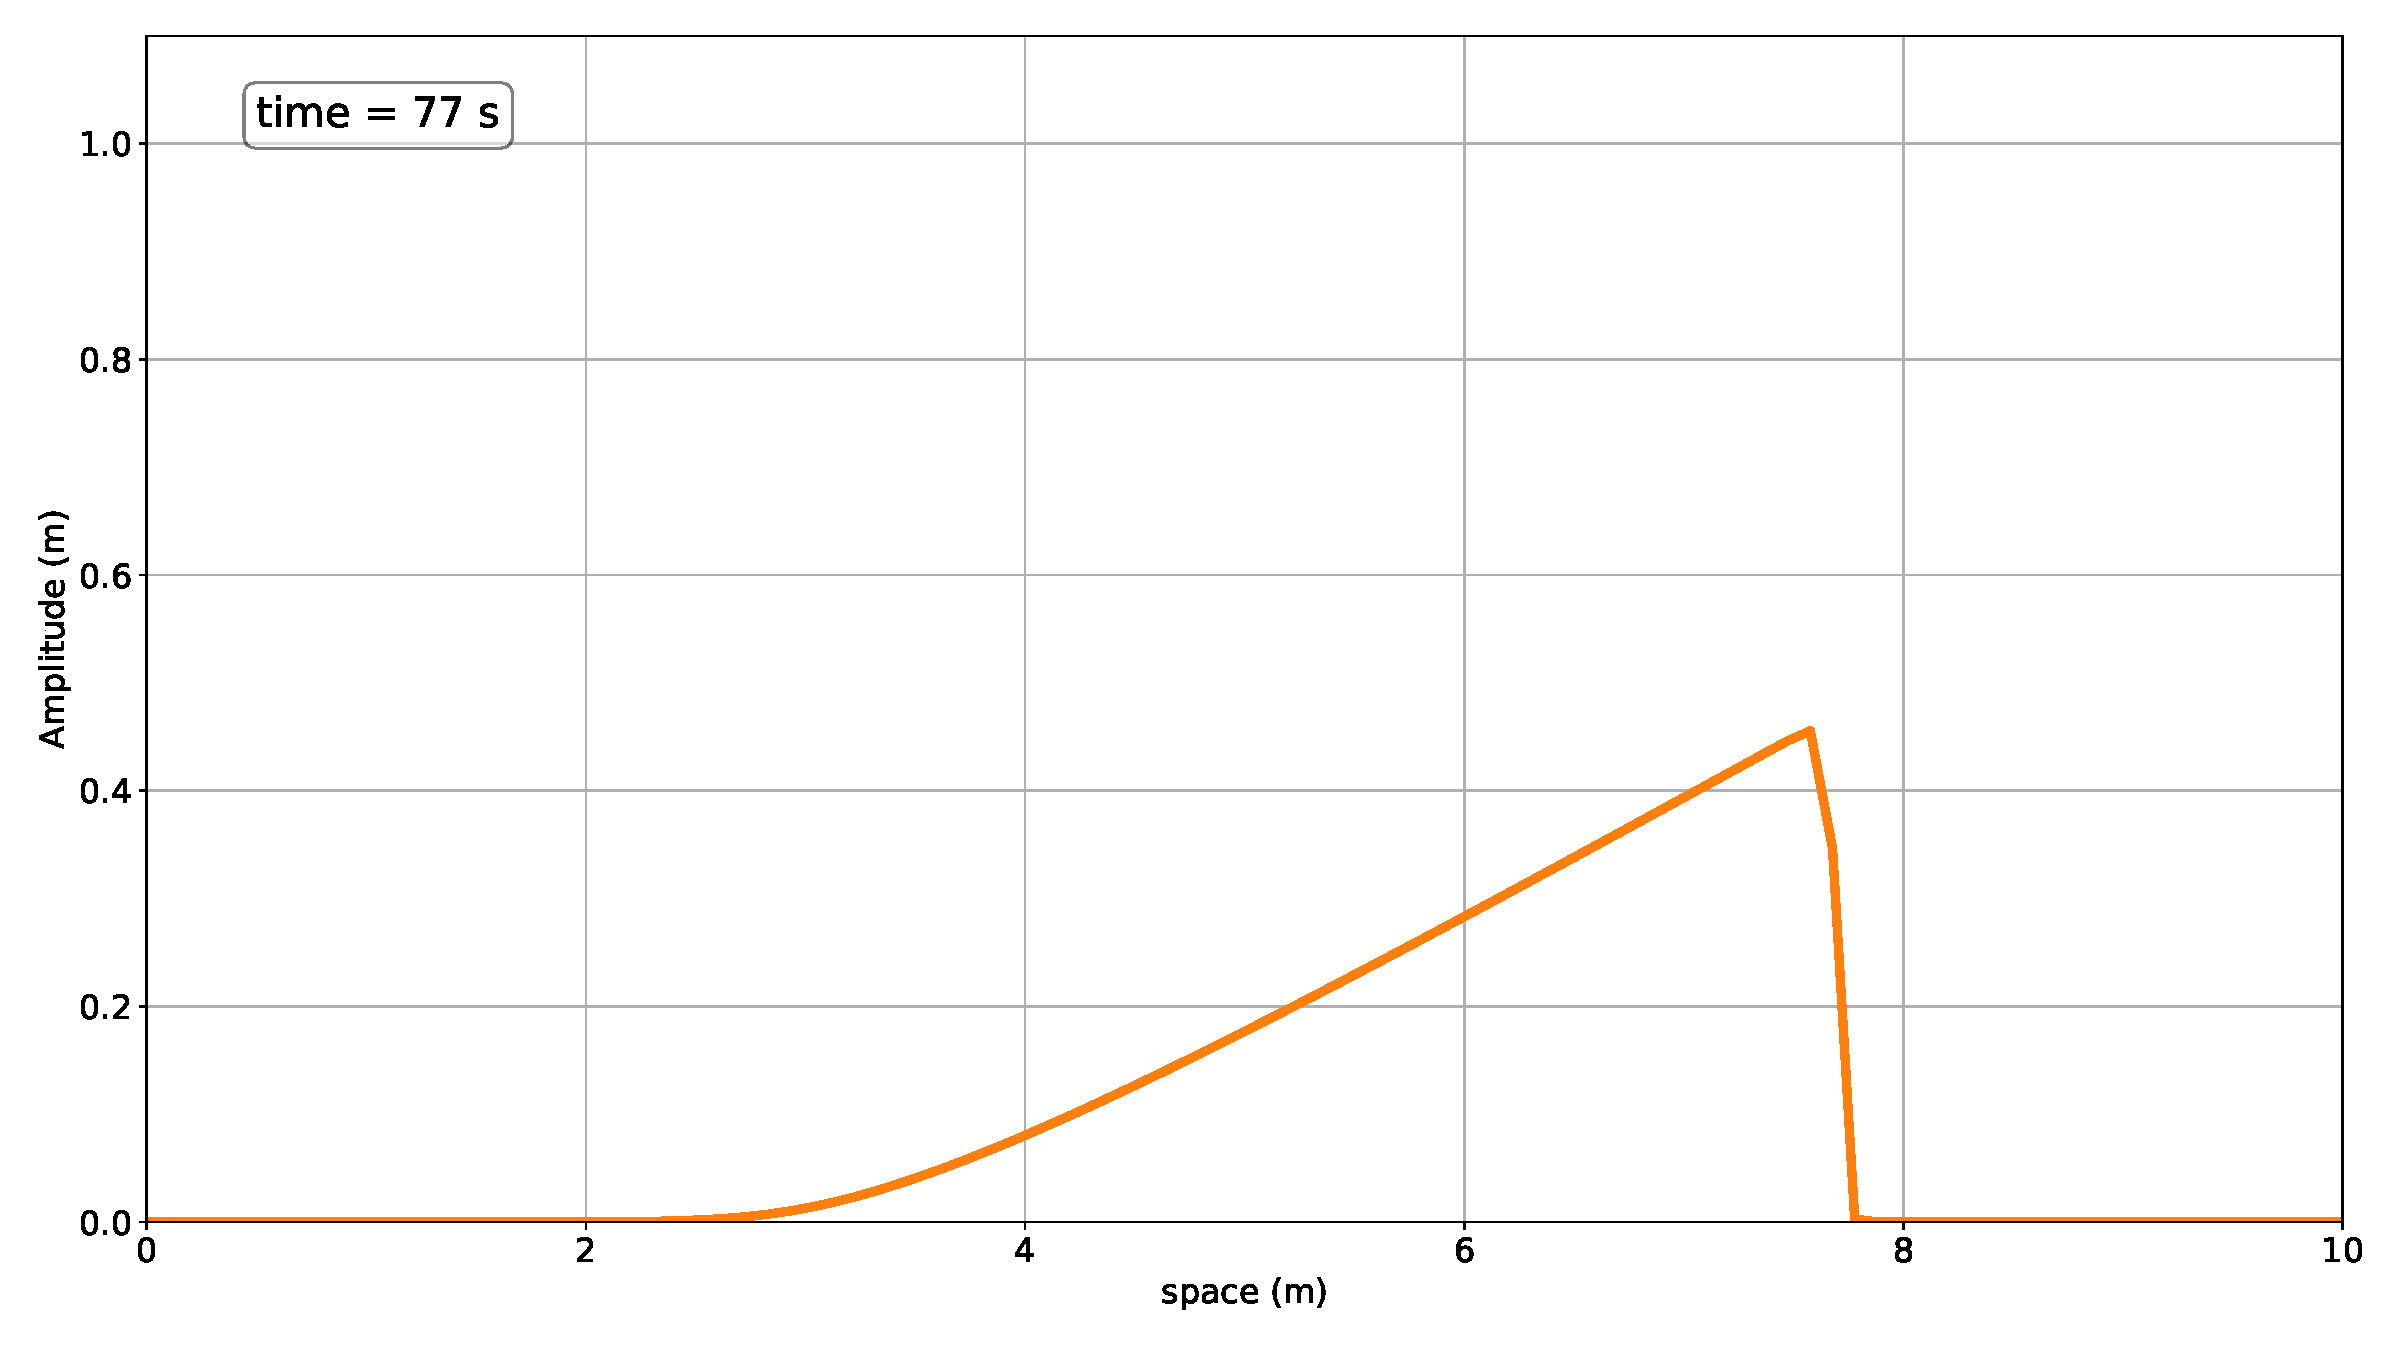
\includegraphics[width=\linewidth]{../BurgersEquation/images/Nonlinear_Convection7.pdf}
% 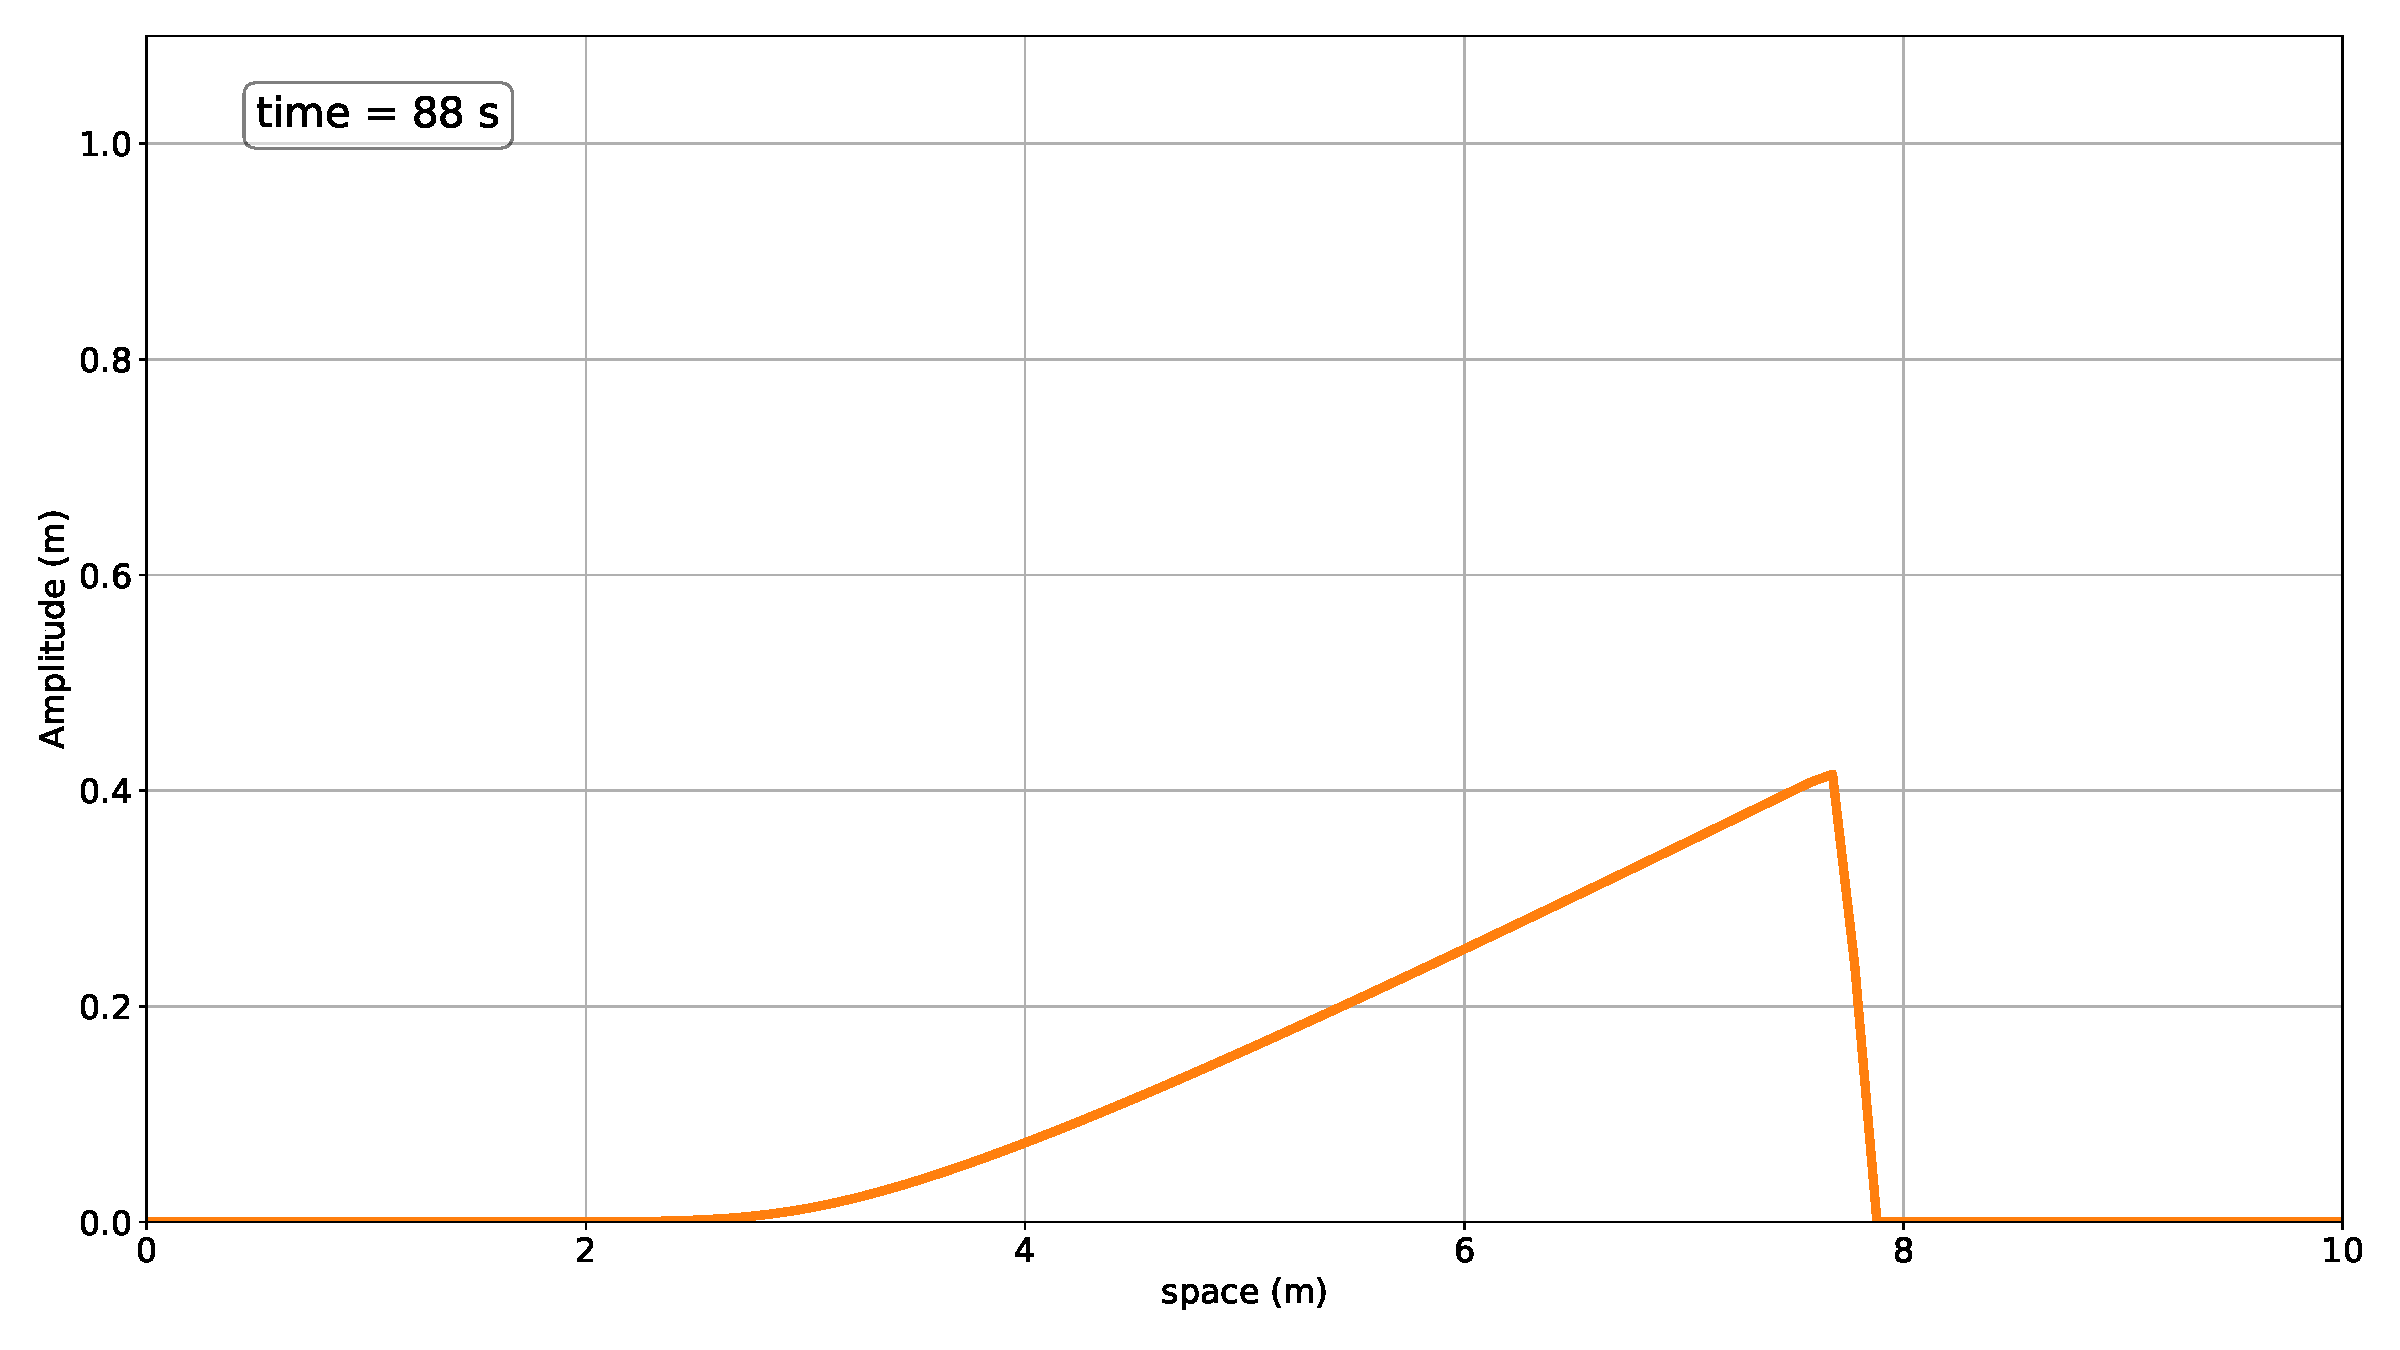
\includegraphics[width=\linewidth]{../BurgersEquation/images/Nonlinear_Convection8.pdf}
% 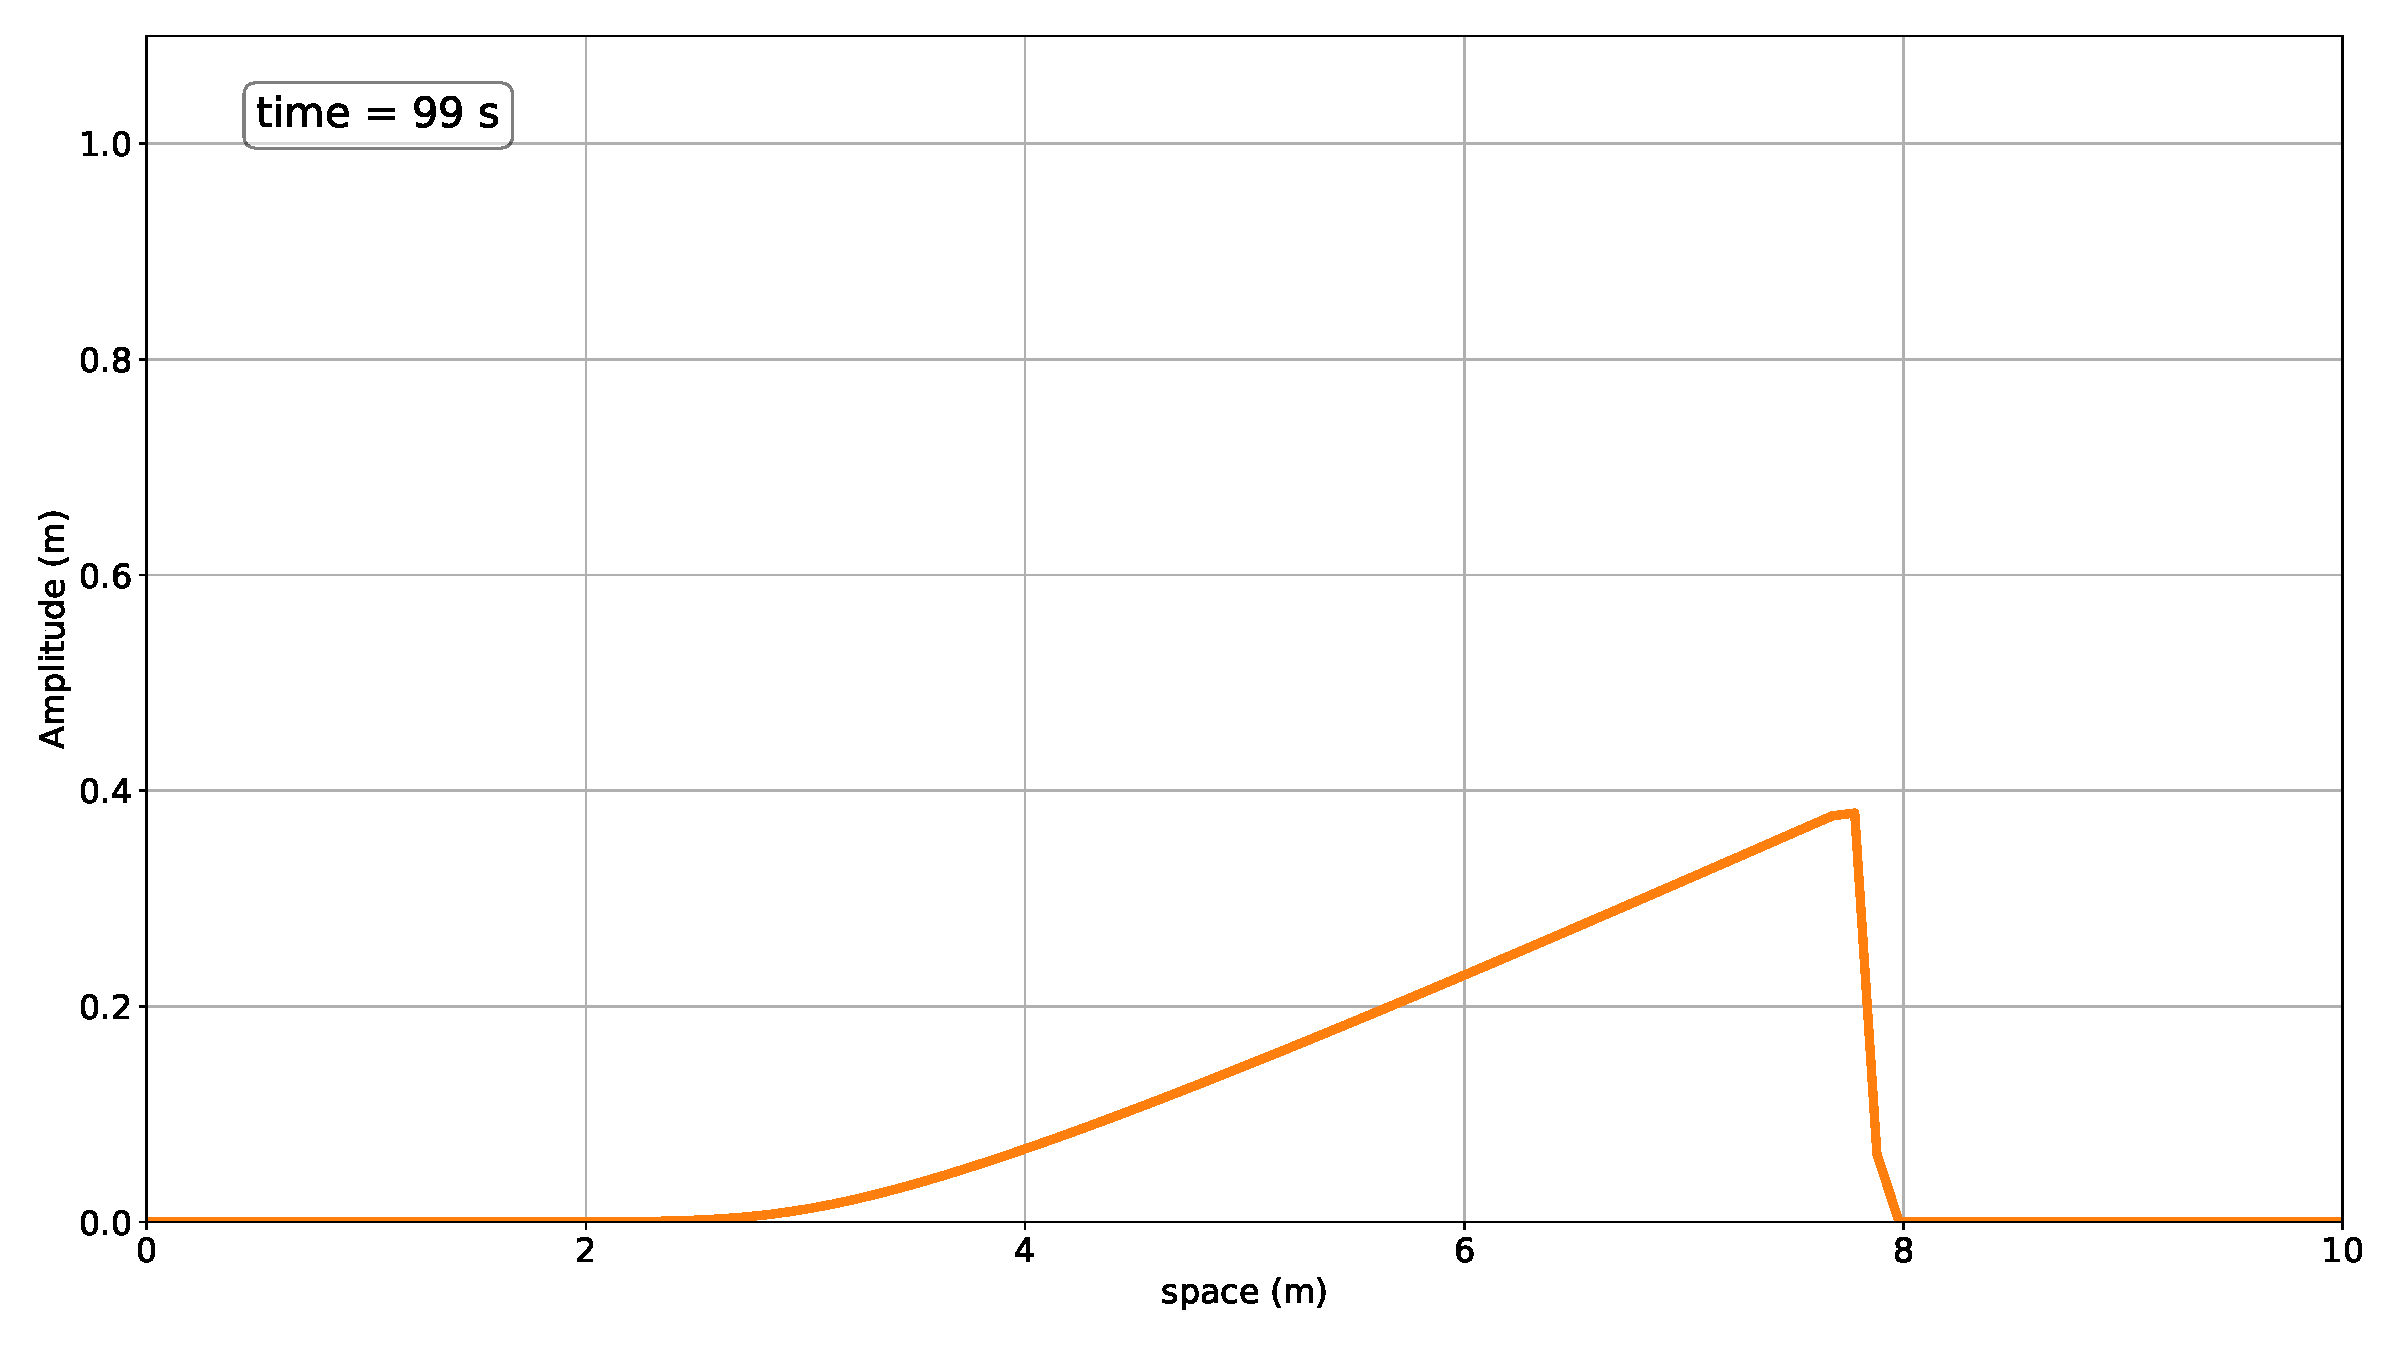
\includegraphics[width=\linewidth]{../BurgersEquation/images/Nonlinear_Convection9.pdf}

\begin{frame}
  \frametitle{Nonlinear Convection aka. Burgers' Equation}
  \begin{columns}
    \column{0.5\linewidth}
    \begin{center}
      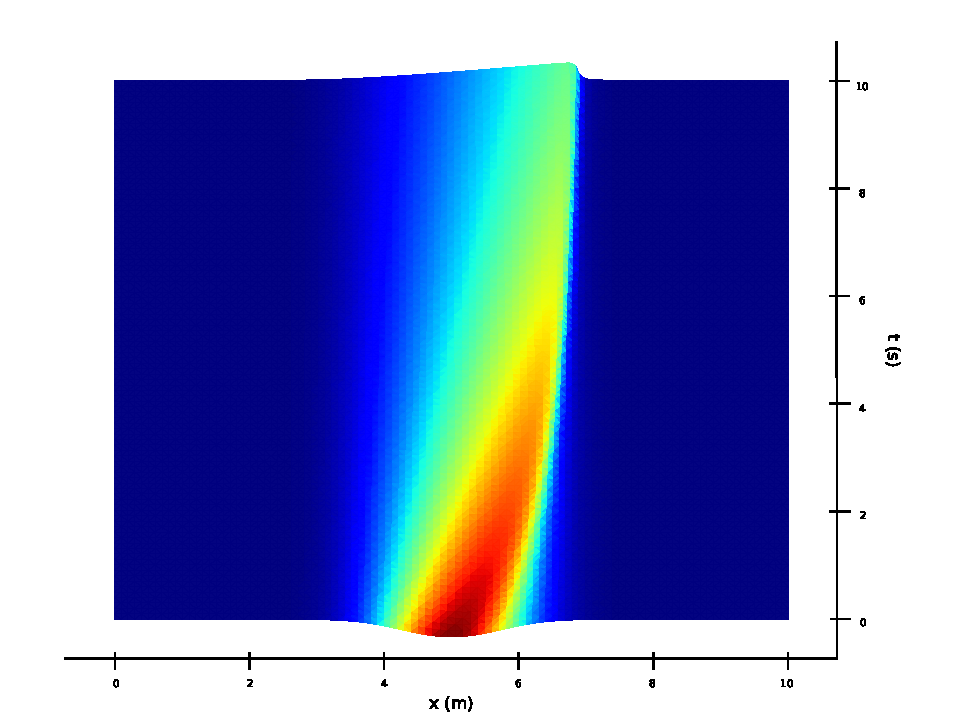
\includegraphics[height=.7\textheight]{../BurgersEquation/images/Implicit_top.pdf}
    \end{center}
    \column{0.5\linewidth}
    \begin{center}
      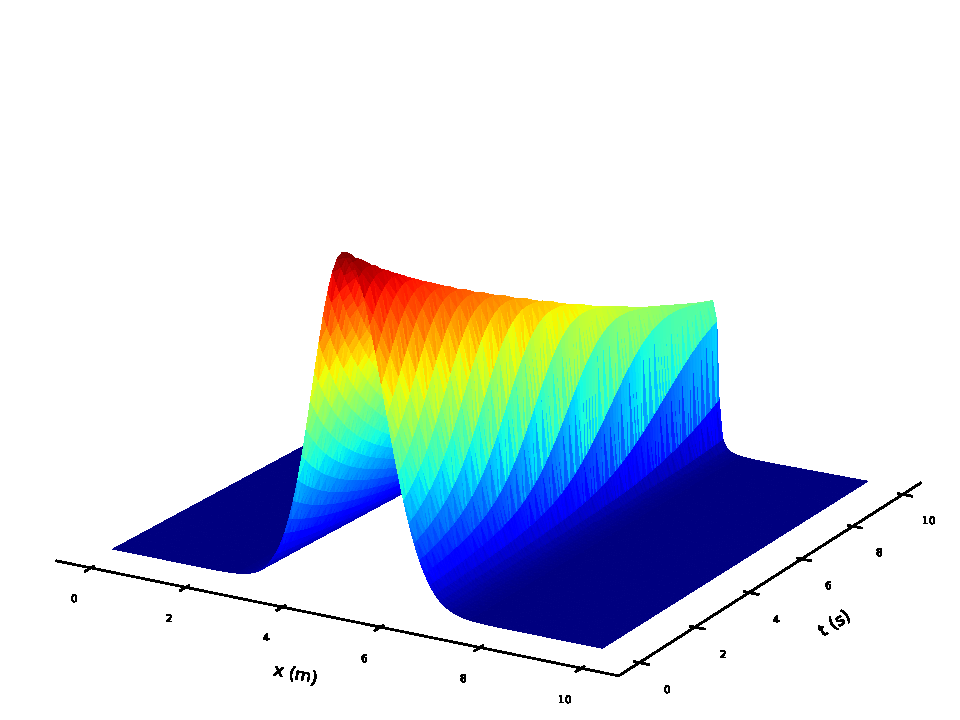
\includegraphics[height=.7\textheight]{../BurgersEquation/images/Implicit_front.pdf}
    \end{center}
  \end{columns}
\end{frame}

% \includegraphics[width=\linewidth]{../Burgers equation/images/Nonlinear_Convection_thumb.pdf}
